% !TEX root = ../Poissons.tex


\subsection{Operadic diagonals for the permutahedra}

We consider the unordered sets $$U(n)  \eqdef  \set{\{I,J\}}{I,J \subset [n], |I|= |J|, I\cap J = \emptyset} \ . $$

\begin{definition}
The $\LA$ and $\SU$ orders on $U=\{U(n)\}$ are defined by 
\begin{itemize} 
    \item $\LA(n) \eqdef \set{(I,J)}{\{I,J\} \in U(n), \ \min(I\cup J) = \min I}$, and by 
    \item $\SU(n) \eqdef \set{(I,J)}{\{I,J\} \in U(n), \ \max(I\cup J) = \max J}$.
\end{itemize}
\end{definition}

As we have seen in the preceding Section, the $\LA$ order defines the diagonal $\LAD$. 
Similarly, we will show in \Guillaume{Corollary X} that the $\SU$ order defines the Saneblidze--Umble diagonal from $\SUD$ \cite{SaneblidzeUmble04}.
Both of these diagonals have opposites $(\LAD)^{\op}$ and $(\SUD)^{\op}$, obtained by permuting the factors in every term; at the level of orderings they are obtained by permuting $I$ and $J$ in the definitions of $\LA(n)$ and $\SU(n)$. 
Geometrically, these opposite versions are given by taking $-\vec v$ instead of $\vec v$ as an orientation vector. 

In general, an \emph{ordering} $O$ of $U$ is a family of sets $\{O(n)\}_{n\geq 1}$ where each $O(n)$ has as elements ordered pairs $(I,J)$ or $(J,I)$, for each $\{I,J\} \in U(n)$.
For an ordered pair $(I,J)$ in $O(n)$, we denote by $\std(I,J)$ the standardisation function, e.g. $\std(\{5,9,10\},\{6,8,12\}) = (\{1,4,5\},\{2,3,6\})$.

\begin{definition}
    \label{def:operadic-ordering}
An ordering $O \eqdef \{O(n)\}_{n \geq 1}$ of $U \eqdef \{U(n)\}_{n\geq 1}$ is \emph{operadic} if for all $(I,J) \in O$, we have that $(I',J') \subsetneq (I,J) \implies \std(I',J') \in O$. 
\end{definition}

We will see \Guillaume{in prop X} that these choice of orderings induce operadic structure on the operahedra, multiplihedra and associahedra.

\begin{lemma} \label{lem:operadic-ordering}
The $\LA$ and $\SU$ orderings are operadic, and are extensions of the following $(I,J)$ pairs,
\begin{itemize}
    \item $\LA :$ for all $k\geq 1$  $(\{1,k+2,k+3,\dots,2k-1,2k\}, \{2,3,\dots,k+1\})$, and 
    \item $\SU :$ for all $k\geq 1$  $(\{k,k+1,\dots,2k-1\},\{1,2,3,\dots,k-1,2k\})$. 
\end{itemize}
The dual orders $\LA^{op}$ and $\SU^{op}$ are also operadic, and extensions of the opposite pairs.
\end{lemma}

\begin{proof}
We present the proof for the $\LA$ ordering, the proofs for the $\SU$ and opposite orders are similar.
First, observe that if an ordered pair $(I,J)$ can be written as $(I_a \sqcup I_b, J_a \sqcup J_b)$ with $(I_a,J_a)$ and $(I_b,J_b)$ in $\LA(|I|)$, then $(I,J)$ is itself in $\LA$.
Second, it is apparent that $(I_k,J_k) \eqdef (\{1,k+2,k+3,\dots,2k-1,2k\}, \{2,3,\dots,k+1\})$ is not a union of other $\LA$ pairs as $1$ is the only element of $I_k$ which is smaller than other elements of $J_k$.
As such, if we try to decompose $(I_k,J_k)$ as a non-trivial union, there is always one pair $(I,J)$ in this union for which $1 \notin I$, so we have $\min ( I \cup J) = \min J$, which implies that $(I,J) \notin \LA$.
Third, we show that any pair $(I,J)$ in $\LA$ which is not of the form $(I_k,J_k)$ can be decomposed as a union of such pairs. 
In combination with the two previous observations, this will prove the Lemma. 

Let $(I,J)$ be in $\LA(k)$ and suppose that $(I,J) \neq (I_k,J_k)$, then there exists $i_2 \in I\ssm \min I$ such that $i_2 < \max J$.
This means that $(I,J)$ can be decomposed as a union: if we write it as $(\{i_1,\dots,i_k\},\{j_1,\dots,j_k\})$, where each set ordered smallest to largest, then we must have $1=i_1<i_2<j_k$, in which case $(\{i_2\},\{j_k\})$ and $(\{i_1,i_3,\dots,i_k\},\{j_1,\dots,j_{k-1}\})$ are both smaller $\LA$ pairs.
Then it must be the case that $\std((\{i_2\},\{j_k\})) = (\{1\},\{2\})$, and $\std((\{i_1,i_3,\dots,i_k\},\{j_1,\dots,j_{k-1}\}))$ is either $(I_{k-1},J_{k-1})$, or we can repeat this decomposition.
This process must eventually terminate with the right-hand side reducing to $(I_l,J_l)$ for some $1 \leq l \leq k-1$.
In other words, any $(I,J) = (\{i_1,\dots,i_k\}, \{j_1,\dots,j_k\})$ decomposes as
\begin{align*}
	(I,J) = (\{i_2\},\{j_k\}) \sqcup (\{i_3\},\{j_{k-1}\}) \sqcup \dots \sqcup (\{i_{l+1} \},\{j_{k-l-1} \}) \sqcup (I',J')
\end{align*}
where $\std((I',J')) = (I_l,J_l)$, and $1\leq l \leq k$.
\end{proof}

We note that the decomposition in \cref{lem:operadic-ordering} is one of potentially many different decompositions of the pair $(I,J)$. 
However, by definition of the $\LA$ order, for any decomposition $(I,J) = (\sqcup_{a\in A} I_a, \sqcup_{a \in A} J_a)$, we have that $\forall a \in A, \std(I_a, J_a) \in \LA$.
As such all decompositions of a pair $(I,J)$ order it the same way.

\begin{proposition}
    \label{prop:operadic-ordering}
The only operadic orderings of $U=\{U(n)\}_{n\geq 1}$ are the $\LA,\SU,\LA^{\op}$ and $\SU^{\op}$ orderings.
\end{proposition}

\begin{proof}
We first observe that there are precisely four ways to order the $U(n)$ pairs of size $k\leq 2$ such that the coherent extension of these orders do not collide.
These are,
\begin{itemize} 
    \item $(\{1\},\{2\})$ and $(\{1,4\},\{2,3\})$ which corresponds to $\LA$ i.e. $\min(I\cup J) = \min I$;
    \item $(\{1\},\{2\})$ and $(\{2,3\},\{1,4\})$ which corresponds to $\SU$ i.e. $\max(I\cup J) = \max J$;
    \item $(\{2\},\{1\})$ and $(\{2,3\},\{1,4\})$ which corresponds to $\LA^{\op}$ i.e. $\min(I\cup J) = \min J$;
    \item $(\{2\},\{1\})$ and $(\{1,4\},\{2,3\})$ which corresponds to $\SU^{\op}$ i.e. $\max(I\cup J) = \max I$.
\end{itemize}
More specifically, we must first order the sole reduced pair $\{\{1\},\{2\}\}$ of $U(1)$.
Then, the sole reduced pair of $U(2)$ which must be ordered is $\{\{1,4\},\{2,3\} \}$.
There are clearly four ways to order these two pairs, and we can identify these $(I,J)$ pairs as cases of \cref{lem:operadic-ordering}.

We now show that once we have committed to one of these four orders we must follow through with it.
We will show this through induction for the $LA$ order, the $\SU$ and opposite orders proceeds similarly.
Let $l\geq 2$ and suppose that for all $k\leq l$, we have ordered $I_k=\{1,k+2,k+3,\dots,2k-1,2k\} < J_k=\{2,3,\dots,k+1\}$.
Then from \cref{lem:operadic-ordering} we know that the only $\{I,J\}$ pair of order $l+1$ that will not decompose (and hence be specified by the already chosen conditions) is $\{I_{l+1},J_{l+1}\}$.
As such, the only way we can vary from $\LA$ is to order this element in the opposite direction i.e. choose $(J_{l+1},I_{l+1})$.
However, this choice leads to contradictions in the ordering of the $\{I,J\}$ pairs of order $|I|=|J|=l+2$.
The following is a generalisation of \cref{ex:Non-coherent order contradiction}.
For $m = l+2$, the pair $\{I_m,J_m\}$ can be oriented in both directions.
On the one side, we can write $\{I_m,J_m\} = \{I_a \cup I_b, J_a \cup J_b\}$ with $I_a \eqdef  \{1,m+3,\dots,2m\} > J_a \eqdef  \{4,5,\dots,m+2\}$  and $I_b \eqdef \{3\} > J_b \eqdef  \{2\}$, which imply that $I_m > J_m$ by the first remark in the proof of \cref{lem:operadic-ordering}. 
This decomposition makes use of the (reversed) order $J_{l+1} > I_{l+1}$ and the (non-reversed) order $I_1 < J_1$.
On the other side, we can write $\{I_m,J_m\} = \{I_c \cup I_d, J_c \cup J_d\}$, where $I_c \eqdef  \{1,m+3,\dots,  2m-1\} < J_c \eqdef  \{2,5,\dots,m+1\}$ and $I_d \eqdef \{3, 2m\} < J_d \eqdef  \{4, m+2\}$, which imply that $I_m < J_m$ via the (non-reversed) orders $I_l < J_l$ and $I_2 < J_2$, a contradiction.
\end{proof}

\begin{example} 
\label{ex:Non-coherent order contradiction}
Suppose that the $\LA$ order holds for pairs of order $1$ and $2$, but is reversed for pairs of order $3$, i.e. we have 
\begin{align*}
    \{1\}<\{2\},\quad \{1,4\}< \{2,3\}, \text{ and } \{1, 5, 6 \} > \{2, 3, 4\} \ .
\end{align*}
Then $\{I,J\}=\{\{1, 3, 7, 8\}, \{2, 4, 5, 6\}\}$ admits two different orientations.
In particular, 
\begin{align*}
    \{1, 7, 8\} > \{ 4, 5, 6 \} \text{ and } \{3\} > \{2\} &\implies \{1, 3, 7, 8\} >\{2, 4, 5, 6\} \ \text{and} \\
    \{1, 7\}< \{2, 5\} \text{ and } \{3, 8\}< \{4, 6\} &\implies \{1, 3, 7, 8\} <\{2, 4, 5, 6\} \ .
\end{align*}
\end{example}

Now recall that each face $A_1 | \ldots | A_k$ of the permutahedron $P_{|A_1|+\cdots + |A_k|-1}$ is isomorphic to the product $P_{|A_1|-1} \times \cdots \times P_{|A_k|-1}$ of lower dimensional permutahedra, via the isomorphism
\begin{equation*}
    \begin{matrix}
        \Theta & : & \R^{|A_1|} \times \cdots \times \R^{|A_k|} & \overset{\cong}{\longrightarrow} & \R^{|A_1|+\cdots+|A_k|} \\
         & & (x_1,\ldots,x_{|A_1|}) \times \cdots \times (x_{|A_1|+\cdots +|A_{k-1}|+1}, \ldots, x_{|A_1|+\cdots +|A_k|})  & \mapsto & (x_{\sigma^{-1}(1)},\ldots,x_{\sigma^{-1}(|A_1|+\cdots +|A_k|)})
    \end{matrix}
\end{equation*}
where $\sigma$ is the $(|A_1|,\ldots,|A_k|)$-shuffle sending the increasingly ordered elements of~$A_1 \cup \ldots \cup A_k$ to the block by block increasingly ordered elements of $A_1 | \ldots | A_k$.
Note that this map is a particular instance of the eponym map introduced in Point (5) of \cite[Prop. 2.3]{LA21}.

\begin{remark}
    This fact underlies a \emph{permutadic} structure \cite{LodayRonco11,MARKL2020105277}.
\end{remark}

A \emph{diagonal of the permutahedra} $\triangle:=\{\triangle_n\}$ is a family of diagonals $\triangle_n : P_n \to P_n \times P_n$, for each $n$-permutahedron $P_n$, $ n \geq 1$. 

\begin{definition}
    A diagonal of the permutahedra $\triangle$ is \emph{operadic} if for every face $A_1 | \ldots | A_k$ of the permutahedron $P_{|A_1|+\cdots + |A_k|-1}$, the map $\Theta$ induces a topological cellular isomorphism \[  \triangle(A_1) \times \ldots \times \triangle(A_k) \cong \triangle(A_1 | \ldots | A_k) \ . \]
\end{definition}
In other words, we require that the diagonal $\triangle$ commutes with the map $\Theta$, see \cite[Section 4.2]{LA21}.
At the algebraic level, this property is called ``comultiplicativity" in \cite{SaneblidzeUmble04}.
\Guillaume{Our choice of terminology comes from the results in Section X}
Note that in particular such an isomorphism respects the poset structures. 

\begin{theorem}
\label{prop:unique-operad}
There are exactly four operadic diagonals on the permutahedra. 
\end{theorem}

\begin{proof}
    First, by \cite[Theorem 3.9]{LA21} any diagonal in the sense of \cref{def:diagonal} is given by a choice of ordering of $U$.
    Second, every operadic diagonal satisfies \cite[Proposition 4.14]{LA21}, which amounts precisely to an operadic ordering of $U$ in the sense of \cref{def:operadic-ordering}.
    We conclude with \cref{prop:operadic-ordering}.
\end{proof}

The orientation vectors $\vec v=(v_1,\ldots,v_{n}) \in \R^n$ inducing each of these four diagonals are given by the conditions \[ \sum_{i \in I} v_i > \sum_{j \in J} v_j \ , \ \forall (I,J) \in O(n) \ , \]
where $O(n)$ stands for either $\LA(n), \LA(n)^\op, \SU(n)$ or $\SU(n)^\op$.

\begin{remark}
    This answers by the negative a conjecture regarding unicity of diagonals on the permutahedra, raised at the beginning of \cite[Section 3]{SaneblidzeUmble04}, and could be seen as a ``corrected" version of it. \Guillaume{See the next section where we prove that SU diagonal is SU diagonal}
\end{remark}

%%%%%%%%%%%%%%%%%%%%%%%%%%%%%%%%%%%%%%%%%%%%%%%%%%%%%%%%%%%

\subsection{Isomorphisms between permutahedra's operadic diagonals}

Let $P$ be a centrally symmetric polytope, and let $s : P \to P$ be its involution, given by taking a point $p \in P$ to its reflection $s(p)$ with respect to the center of symmetry of $P$. 
Note that this map is cellular, and induces an involution on the face lattice of $P$. 
For $P$ the permutahedron, this face poset involution is given by the assignment $A_1 | \cdots | A_k \mapsto A_k | \cdots | A_1$. 

The permutahedron possesses another symmetry: the cellular involution $r : P \to P$ which sends a point $p \in P$ to its reflection with respect to the hyperplane of equation \[ \sum_{i=1}^{\lfloor n/2 \rfloor}x_i = \sum_{i=1}^{\lfloor n/2 \rfloor}x_{n-i+1} \ . \]
This involution also respects the face poset structure. 
In terms of ordered partitions, it replaces each block $A_j$ in $A_1 | \cdots | A_k$ by the block $r(A_j):=\{n-i+1 \ | \ i \in A_j\}$.

As we have already remarked \Guillaume{in Rem X}, the polytope of diagonals of $P$ is always centrally symmetric, and the involution $t : P \times P \to P \times P$ sending $(x,y)$ to~$(y,x)$ takes a cellular diagonal to another cellular diagonal.
In the case of the permutahedron it sends $\LAD$ to $(\LAD)^\op$ and $\SUD$ to $(\SUD)^\op$.

\begin{theorem}
    \label{thm:bijection-operadic-diagonals}
    For $P$ the permutahedron, the involutions $t$ and $rs \times rs$ are cellular isomorphisms between the four operadic diagonals, through the following commutative diagram: 
    \begin{center}
        \begin{tikzcd}
        \LAD \arrow[r,"t"] \arrow[d,"rs \times rs"]&
        (\LAD)^{\op}\arrow[d,"rs \times rs"]\\
        \SUD \arrow[r,"t"] &
        (\SUD)^\op
        \end{tikzcd}
        \end{center}
    Moreover, they induce poset isomorphisms at the level of the face lattices. 
\end{theorem}

\begin{proof}
    The result for the transpositions $t$ and the commutativity of the diagram are straighforward, so we prove that $rs\times rs$ is a cellular isomorphism respecting the poset structure. 
    First, we observe that the assignment $(I,J) \mapsto (r(J),r(I))$ defines a bijection between $\LA(n)$ and $\SU(n)$. 
    Indeed, we have $r(\min(I\cup J))=\max(I\cup J)$; since $I \cap J = \emptyset$, $r$ is well-defined, and it is a bijection with inverse $r$ itself.  
    Denoting by $N^c$ the complement of a subset $N \subset [n]$, we have that $|N \cap I| > |N\cap J| \iff |N^c \cap I|< |N^c \cap J|$.
    Combining this with the fact that $|N \cap I| > |N\cap J| \iff |r(N) \cap r(I)| > |r(N) \cap r(J)|$, we obtain that 
    \begin{eqnarray*}
        |N \cap I| > |N\cap J| \iff |r(N)^c \cap r(I)| < |r(N)^c \cap r(J)| \ .
    \end{eqnarray*}
    Similarly, we have $|N' \cap I| < |N'\cap J| \iff |r(N')^c \cap r(I)| > |r(N')^c \cap r(J)|$, so that $(\sigma,\tau) \in \LAD$ if and only if $(rs(\sigma),rs(\tau)) \in \SUD$. 
    Finally, since both $t,r$ and $s$ preserve the poset structures, so does their composition, which finishes the proof.
\end{proof}

\begin{remark}
    There is a second, distinct isomorphism given by $t(r\times r)$ \Guillaume{TBC}
\end{remark}

%%%%%%%%%%%%%%%%%%%%%%%%%%%%%%%%%%%%%%%%%%%%%%%%%%%%%%%%%

\subsection{Facets of operadic diagonals}

We have seen in \cref{thm:vertices2nBraidArrangement} that facets of any diagonal of the permutahedron are in bijection with $(2,n)$-trees, that is pair of partitions whose intersection graph is a tree.
These are precisely the \emph{essential complementary partitions} studied in \cite{chen1969computer,chen1971tables,kajitani1982number}. 
Here we describe a specific planar embedding of the $(2,n)$-trees for each operadic diagonal. 
\Guillaume{Simplify and unify exposition with Section 1}

\begin{definition}
A set of \emph{distinct representatives} of an (unordered) partition $\sigma_I$ is a set $M\subset [n]$ such that $\forall i \in I,|\sigma_i \cap M| = 1$.
\end{definition}

\begin{definition}
A pair of partitions $(\sigma_L,\tau_R)$ is 
\begin{enumerate} 
    \item \emph{complementary} if there exists $M\subset [n]$ and $m \in M$ such that $M$ and $([n]\ssm M) \cup \{m\}$ are distinct representatives of $\sigma_L$ and $\tau_R$, respectively,
    \item it is furthermore \emph{essential} if there does not exist proper subsets $ L'\subset L$, $R'\subset R$ and $N \subset [n]$ such that $(\sigma_{L'},\tau_{R'})$ is a complementary partition of $N$.
\end{enumerate}
\end{definition}

An equivalent definition is the following. 

\begin{definition}
A pair of partitions $(\sigma_L,\tau_R)$ is said to be 
\begin{enumerate}
	\item \emph{complementary}, if $\forall l\in L, r\in R$ we have that $|\sigma_l \cap \tau_r| \leq 1$,
	\item \emph{essential}, if there are no proper subsets of $L'\subset L,R'\subset R$ such that $\cup_{l \in L'} \sigma_l = \cup_{r \in R'} \tau_r$.
\end{enumerate}	
\end{definition}

In cases where there is no ambiguity we will drop the subscripts $L,R$.
We shall denote the set of all essential complementary pairs of partitions of $[n]$ by $\EC$.
Let us emphasize that the pairs of partitions of $\EC$ are \emph{unordered}.

\begin{example}
For $n=2$, the two essential complementary partitions are $1|2 \times 12$ and $12 \times 1|2$. For $n=3$, the eight essential complementary partitions are
\begin{align*}
	1|2|3 \times 123,\quad 
	123 \times 1|2|3,\quad 
	1|23 \times 13|2,\quad 
	13|2 \times 1|23\\
	1|23 \times 12|3,\quad 
	12|3 \times 1|23,\quad 
	13|2 \times 12|3,\quad 
	12|3 \times 13|2
\end{align*}
For a larger example see \cref{ex:ECbijection}. 
\end{example}

%A \emph{tree} is a simply connected graph with no cycles. 
%A \emph{bipartite graph} is a graph whose vertices are partitioned into two sets such that vertices in one set are only adjacent to vertices in the other.
%We say a bipartite graph is \emph{ordered} if one of the sets is considered smaller than the other and we denote the partition $(V_L,V_R)$. 
%We say a graph with $n$ edges is \emph{edge labelled} if there exists a bijection between the edges and $\{1,\dots,n\}$.

As we have seen in the proof of \cref{thm:vertices2nBraidArrangement}, essential complementary partitions are in bijection with $(2,n)$-trees.
Given an essential complementary pair $(\sigma,\tau)$, the corresponding $(2,n)$-tree has the blocks of each partition as its vertices, and two such vertices are connected by an edge if the two blocks share a common element, which labels the edge, see \cref{ex:ECbijection}.


\begin{theorem}
\label{thm:facets}
The facets of any operadic diagonal $\OP$ are in bijection with essential complementary partitions, through the inverse functions $u:\OP \to \EC$ and $o:\EC\to \OP$, where
\begin{enumerate}
    \item the function $u$ forgets the order of the ordered partition pair,
    \item the function $o$ uniquely orders an essential complementary partition pair via the minimal $(I,J)$-pairs defining the diagonal. 
\end{enumerate}
In particular, this defines a particular planar embedding of each $(2,n)$-tree, as illustrated in \cref{ex:ECbijection}.
\end{theorem}

We shall prove this theorem by establishing the necessary total order, showing that the functions are well defined, and then showing that they are injective.
We will work with the $\LAD$ diagonal, but the proofs can be straightforwardly modified to accomodate any of the other three operadic diagonals. 

\begin{lemma} 
\label{l:u-well-defined}
The function $u:\OP \to \EC$ that forgets the order in a pair of partitions is well defined.
\end{lemma}
\begin{proof}
Let $(\sigma,\tau)$ be a pair of ordered partitions forming a facet of $\LAD$. 
Their intersection graph has $n+1$ vertices and $n$ edges, and as no vertices can be isolated it must be a tree. 
%It is straightforward to verify that it must be a labeled bipartite tree, but here is how we may explicitly produce the necessary distinct representatives using an algorithm of \cite[Theorem 2]{kajitani1982number}.
%Let $G'$ be a copy of $G(u(P))$. 
%While there is a vertex of degree $1$ in $G'$ delete it and add the sole edge of that vertex as a distinct representative of the corresponding partition of that vertex. 
%As $G'$ is a tree this process can continue until there is a single edge connecting two vertices of degree $1$. 
%This edge specifies the element $p$ of the distinct representatives.
\end{proof}

\begin{construction} 
\label{const:total}
For $(\sigma,\tau) = (\bigcup_{l\in L}\sigma_l,\bigcup_{r\in R} \tau_r)$ an essential complementary pair, we construct total orders on the blocks of $\sigma$ and $\tau$ in three steps:
\begin{enumerate}
    \item For any two blocks $\sigma_k,\sigma_l$ in $\sigma$ or $\tau$, there is a unique minimal path $\gamma$ of even cardinality  connecting them.
    We partition $\gamma=I\cup J$ where $\min(I\cup J) \in I$ and the path alternates between elements of $I$ and $J$;
    \item Direct each path $\gamma$ so that all the edges of $I$ (resp. $J$) go from left to right (resp. right to left);
    \item We say $\sigma_k< \sigma_l$ if the path joining them is directed from $\sigma_k$ to $\sigma_l$.
\end{enumerate}
\end{construction}

\begin{proof}
We first show our binary relation is well defined before verifying that it defines a total order on the vertices of the $(2,n)$-tree.
In a bipartite tree, every vertex is connected, and every path connecting two vertices on the same side must be of even length. 
As $I$ and $J$ partition the path in an alternating fashion i.e. $\gamma=(i_1,j_1,i_2,j_2,\dots)$, we can orient it by forcing each edge of $I$ (resp. $J$) to point to the right (resp. left). 
This order is clearly total, reflexive (by convention) and anti-symmetric, what remains to be checked is its transitivity. 

Let $\gamma$ denote the unique maximal path between two vertices $a$ and $b$ on the left of the tree, that is two blocks of $\sigma$. 
Let $I_{ab}$ denote the set of left-to-right edges in this path, and let $J_{ab}$ denote its complement. 
Then, we have 
\begin{equation}
    \label{eq:order}
    a < b \iff \min(I_{ab}\cup J_{ab})=\min(I_{ab}) \ . 
\end{equation}
Suppose now that $a < b$ and $b < c$.
Since $\gamma_{ac}= (\gamma_{ab} \cup \gamma_{bc}) \ssm (\gamma_{ab} \cap \gamma_{bc})$, we have $$ I_{ac}=(I_{ab}\cup I_{bc}) \ssm (J_{ab} \cup J_{bc}) \text{ and } J_{ac}=(J_{ab}\cup J_{bc}) \ssm (I_{ab} \cup I_{bc}) \ , $$ and from the condition (\ref{eq:order}) above it is clear that $\min(I_{ac}\cup J_{ac})=\min(I_{ac})$, which completes the proof of the transitivity for the total order on $\sigma$. 
The proof for $\tau$ is similar. 
\end{proof}

\begin{example}
\label{ex:ECbijection}
We now illustrate the ordering (right) of the pair of essential complementary partitions $\{15,234,6,7\} \times \{13,2,46,57\}$ (left).
\begin{center}
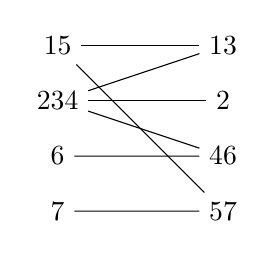
\begin{tikzpicture}[scale=.7]  
\node (1) at (-1.5, -1) {$15$};
\node (2) at (-1.5, -2) {$234$};
\node (3) at (-1.5, -3) {$6$};
\node (4) at (-1.5, -4) {$7$};
%
\node (5) at (1.5, -1) {$13$};
\node (6) at (1.5, -2) {$2$};
\node (7) at (1.5, -3) {$46$};
\node (8) at (1.5, -4) {$57$};
%
\draw[-] (1)--(5); 
\draw[-] (1)--(8);
\draw[-] (2)--(5); 
\draw[-] (2)--(6); 
\draw[-] (2)--(7); 
\draw[-] (3)--(7);
\draw[-] (4)--(8);
%
\end{tikzpicture}
$\quad$
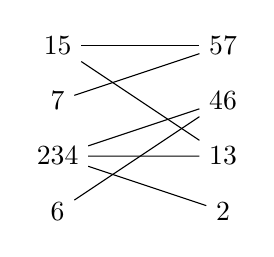
\begin{tikzpicture}[scale=.7]  
\node (1) at (-1.5, -1) {$15$};
\node (2) at (-1.5, -2) {$7$};
\node (3) at (-1.5, -3) {$234$};
\node (4) at (-1.5, -4) {$6$};
%
\node (5) at (1.5, -1) {$57$};
\node (6) at (1.5, -2) {$46$};
\node (7) at (1.5, -3) {$13$};
\node (8) at (1.5, -4) {$2$};
%
\draw[-] (1)--(5); 
\draw[-] (1)--(7);
\draw[-] (2)--(5); 
\draw[-] (3)--(6); 
\draw[-] (3)--(7); 
\draw[-] (3)--(8); 
\draw[-] (4)--(6);
%
\end{tikzpicture}
\end{center}
Here are two examples of paths providing order information, with $(I,J)=(\{1,7\},\{3,5\})$ and $(I,J)=(\{1,4\},\{3,5\})$
\begin{align*}
	7 <_L 234 \text{ as } 7 \xrightarrow{7} 57 \xrightarrow{5} 15 \xrightarrow{1=\min(I\cup J)} 13 \xrightarrow{3} 234 \ , \\
	57 <_R 46 \text{ as } 57 \xrightarrow{5} 15 \xrightarrow{1=\min(I\cup J)} 13 \xrightarrow{3} 234 \xrightarrow{4} 46 \ .
\end{align*}
\end{example}

This order far from being arbitrary provides the unique way to order an essential complementary partition pair into an ordered partition pair of $\LAD$, as we shall demonstrate next.
First we need a geometrical result. 

\begin{proposition}
    \label{prop:geometrical-IJ}
    The paths between adjacents vertices of $\sigma$ or $\tau$ are in bijection with the minimal $(I,J)$-pairs (see \cref{s:diagonals-permutahedra}).
\end{proposition}

\begin{proof}
    By \cref{p:minimal-IJ-pairs}, it suffices to show that the paths between adjacent vertices of $\sigma$ are in bijection with the solutions of the system of equations of the form $(\rho^1,\sigma^2)$. 
    To ease notation let us write $\rho$ for $\rho^1$ and $\sigma$ for $\sigma^1$. 
    Suppose that $\rho$ is obtained from $\sigma$ by merging the two blocks $\sigma_a$ and $\sigma_b$. 
    The two equations $\langle \vec \sigma_a, x \rangle =0$ and $\langle \vec \sigma_b, x \rangle =0$ now become $\langle \vec \sigma_a + \vec \sigma_b, x \rangle =0$; nothing else changes in the system. 
    Since the solution to the system $(\sigma^1,\sigma^2)$ was $x=0$, now the solution is of dimension $1$, and it is given precisely by the path between $a$ and $b$.
    Such a path is given by an alternating sequence of vertices and edges $\sigma_1 \eqdef \sigma_a, e_1, \sigma_2, e_2, \ldots, e_{k-1}, \sigma_k \eqdef \sigma_b$. 
    Every edge $e_i \in \{1,\ldots, n\}$ is by definition the intersection $\sigma_{i} \cap \sigma_{i+1}$; thus it is the only common non-zero coordinate between $\vec \sigma_{i}$ and $\vec \sigma_{i+1}$.
    Thus the path encodes the series of equations $x_{e_1}+x_{e_{k-1}}=0$, $x_{e_1}+x_{e_2}=0$, $x_{e_2}+x_{e_3}=0$, $\ldots$, $x_{e_{k-2}}+x_{e_{k-1}}=0$. 
    Thus, $x_{e_1}=1$, $x_{e_2}=-1$, $x_{e_3}=1$, $\ldots$, $x_{e_{k-2}}=1$, $x_{e_{k-1}}=-1$ is a basis of one-dimensional space of solutions, and it gives the corresponding minimal $(I,J)$-pair. 
\end{proof}

\begin{lemma} 
\label{l:o-well-defined}
The function $o:\EC \to \LAD$ which orders an essential complementary pair is well defined.
\end{lemma}

\begin{proof}
Consider the ordering $o(\sigma,\tau)$ of the pair $(\sigma,\tau)$ given by \cref{const:total}. 
We first show that every $(I,J)$-condition, for $(I,J) \in \LA(n)$, which corresponds to a path between vertices is satisfied. 
In particular, this statement will be true for paths between adjacent vertices, which are exactly the minimal $(I,J)$-pairs according to \cref{prop:geometrical-IJ}.
This will in turn allow us to conclude since testing the minimal $(I,J)$-pairs is equivalent to testing all $(I,J)$-pairs as stated in \cref{p:minimal}. 
Suppose that $I,J$ corresponds to a path between two vertices on the left, i.e.
\begin{align*}
    \sigma_l = \sigma_{l_1} \xrightarrow{i_1} \tau_{r_1}\xrightarrow{j_1} \sigma_{l_2} \xrightarrow{i_2}\dots \xrightarrow{i_{k}} \tau_{r_{k-1}} \xrightarrow{j_k} \sigma_{l_k}= \sigma_{l'}
\end{align*}
By construction we have that $(I = \{i_1,\dots,i_k\},J=\{j_1,\dots,j_k\}) \in \LA(n)$ (note we are ordering $I$ and $J$ by the path, so it is not necessarily the case that $\min I = i_1$). 
Furthermore, each block of $\tau$ either contains a single element of $I$ and a single element of $J$, or it contains no elements of $I$ and no elements of $J$. 
As such for any ordering of the blocks of $\tau$ we have that
\begin{align*}
    \forall m, \bigg|\bigcup_{1\leq k \leq m} \tau_{k} \cap I \bigg| = \bigg|\bigcup_{1\leq k \leq m} \tau_{k} \cap J \bigg| \ .
\end{align*}
Hence in order for this $\LA(n)$ condition to be satisfied it must be the case that for some ordering of the blocks of $\sigma$ we have
\begin{align*}
    \exists m, \bigg| \bigcup_{1\leq k \leq m} \sigma_k \cap I \bigg| > \bigg|\bigcup_{1\leq k \leq m} \sigma_k \cap J \bigg| \ .
\end{align*}
Every block of $\sigma$ excluding $\sigma_l$ and $\sigma_{l'}$ either contains no elements of both $I$ and $J$, or contains a single element of $I$ and a single element of $J$. 
So the only way for the condition to be satisfied is for $\sigma_l$ to come before $\sigma_{l'}$, which is precisely what is required by the total order.
If the sets $(I,J)$ correspond to a path between two vertices on the right
\begin{align*}
    \tau_r = \tau_{r_1} \xrightarrow{j_1} \sigma_{l_1}\xrightarrow{i_1} \tau_{r_2} \xrightarrow{j_2}\dots \xrightarrow{j_{k}} \sigma_{l_{k-1}} \xrightarrow{1_k} \tau_{r_k}=\tau_{r'} \ ,
\end{align*}
then a similar chain of logic implies we must have an ordering of the blocks of $\tau$ such that
\begin{align*}
    \exists m, \bigg|\bigcup_{1\leq k \leq m}\tau_k \cap I\bigg| < \bigg|\bigcup_{1\leq k \leq m} \tau_k \cap J\bigg| \ , 
\end{align*}
and this can only happen if $\tau_r$ comes before $\tau_{r'}$.
\end{proof}

\begin{remark}
    It would be interesting to know if there is a geometrical interpretation of the paths that are not between adjacent vertices. 
\end{remark}

To complete the proof of \cref{thm:facets}, it remains to show that both $u:\LAD \to \EC$ and $o:\EC\to \LAD$ are injective, with the other function being their inverse.

\begin{proof}[{Proof of \cref{thm:facets}}]
The forgetful function $u$ is clearly the inverse to $o$ as forgetting any assigned order will clearly return the original essential complementary partition pair. 
The ordering function $o$ is the inverse to $u$ as it returns the sole ordering of the blocks which is compatible with the $\LA(n)$ conditions.
\end{proof}

So, we have the follow characterisation of facets of the $\LAD$ and $\SUD$ diagonals (the second one being obtained by changing slightly \cref{const:total} according to the definition of the $\SU$ order).
We omit the adaptation for the two opposite diagonals, which is immediate.

\begin{corollary} 
\label{prop:LAD-ordered-EC}
The facets of the $\LAD$ (resp. $\SUD$) diagonal are ordered essential complementary partitions in which the minimal (resp. maximal) element of each path is traversed from left to right (resp. right to left).
\end{corollary}

We illustrate how the bijection $rs\times rs$ from \cref{thm:bijection-operadic-diagonals} relates the two results.

\begin{example}
\label{ex:theta-path-translation}
We apply the bijection $rs\times rs$ to the element of $\LAD$ from \cref{ex:ECbijection}
\begin{center}
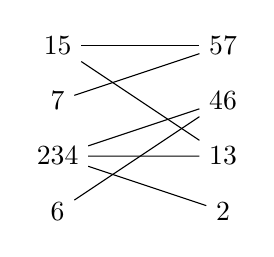
\begin{tikzpicture}[scale=.7]  
\node (1) at (-1.5, -1) {$15$};
\node (2) at (-1.5, -2) {$7$};
\node (3) at (-1.5, -3) {$234$};
\node (4) at (-1.5, -4) {$6$};
%
\node (5) at (1.5, -1) {$57$};
\node (6) at (1.5, -2) {$46$};
\node (7) at (1.5, -3) {$13$};
\node (8) at (1.5, -4) {$2$};
%
\draw[-] (1)--(5); 
\draw[-] (1)--(7);
\draw[-] (2)--(5); 
\draw[-] (3)--(6); 
\draw[-] (3)--(7); 
\draw[-] (3)--(8); 
\draw[-] (4)--(6);
%
\end{tikzpicture}
\quad
\raisebox{3em}{$\xrightarrow{rs\times rs}$}
\quad
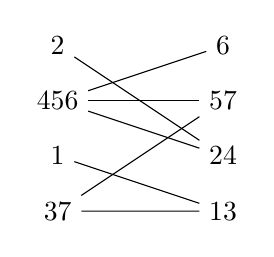
\begin{tikzpicture}[scale=.7]  
\node (1) at (1.5, -4) {$13$};
\node (2) at (1.5, -3) {$24$};
\node (3) at (1.5, -2) {$57$};
\node (4) at (1.5, -1) {$6$};
%
\node (5) at (-1.5, -4) {$37$};
\node (6) at (-1.5, -3) {$1$};
\node (7) at (-1.5, -2) {$456$};
\node (8) at (-1.5, -1) {$2$};
%
\draw[-] (1)--(5);
\draw[-] (1)--(6); 
\draw[-] (2)--(7);
\draw[-] (2)--(8);
\draw[-] (3)--(5); 
\draw[-] (3)--(7);
\draw[-] (4)--(7);
%
\end{tikzpicture} \ .
\end{center}
Observe that the $\LA(7)$ conditions corresponding to paths, such as $( \{1,4\},\{3,5\}) \in \LA(7)$
\begin{align*}
    57 <_R 46 \text{ as } 57 \xrightarrow{5} 15 \xrightarrow{1=\min(I\cup J)} 13 \xrightarrow{3} 234 \xrightarrow{4} 46
\end{align*}
are mapped to $\SU(7)$ conditions corresponding to paths, e.g. the prior $(I,J)$-condition maps to $(r(J),r(I))=( \{3,5 \},\{4,7\}) \in \SU(7)$, and
\begin{align*}
    24 <_R 13 \text{ as } 24 \xrightarrow{4} 456 \xrightarrow{5} 57 \xrightarrow{7=\max(r(J)\cup r(I))} 37 \xrightarrow{3} 13 \ .
\end{align*}
\end{example}
Note that the composite $\LAD \xrightarrow{u} \EC \xrightarrow{o} \SUD$ provides another bijection between facets, however this map is not equal to $rs \times rs$ and is not defined on the other faces.

%%%%%%%%%%%%%%%%%%%%%%%%%%%%%%%%%%%%%%%%%%%%%%%

\subsection{Vertices of operadic diagonals}

We are now interested in characterizing the pairs of vertices that occur in the diagonal, that is pairs of permutations $(\sigma_1,\sigma_2) \in \triangle$. 

\begin{theorem} There exists $(I,J) \in D(n)$ such that $\forall k, |\sigma_1^1\cdots\sigma_1^k \cap I| \leq |\sigma_1^1\cdots\sigma_1^k \cap J|$ and $\forall l, |\sigma_1^1\cdots\sigma_1^l \cap I| \geq |\sigma_1^1\cdots\sigma_1^l \cap J|$ (diagonal condition) if and only if $\exists (I',J')=(\{i_1,\ldots,i_m\},\{j_1,\ldots,j_m\}) \in D(m)$, $m\leq n$, such that \[\sigma_1 \cap (I'\cup J')=j_1 i_1 j_2 i_2 \cdots j_n i_n \] and \[ \sigma_2 \cap (I'\cup J') = i_2 j_1 i_3 j_2 \cdots i_n j_{n-1} i_1 j_n \ , \] where $i_1 = \min (I' \cup J')$ (fish condition). 
\end{theorem}

\begin{proof}
\begin{itemize}
\item If a pair of permutations $(\sigma_1, \sigma_2) \in   \mathfrak{S}_N^2$ satisfies the fish condition, then there exist two sets $I$ and $J$ of same cardinality such that $\min(I)<\min(J)$. Denoting $\sigma_1$ and $\sigma_2$ by two words of size $N$ $\sigma_1^1 \ldots \sigma_1^N$ and $\sigma_2^1 \ldots \sigma_2^N$, then the pair $((\sigma_1, \sigma_2), (I,J))$ satisfies that for any $k$ in $\llbracket 1;N\rrbracket$, $|\sigma_1^1 \ldots \sigma_1^k \cap J| \geq |\sigma_1^1 \ldots \sigma_1^k \cap I|$ and $|\sigma_2^1 \ldots \sigma_2^k \cap I| \geq |\sigma_2^1 \ldots \sigma_2^k \cap J|$, hence the diagonal condition.
\item We will now prove the converse. Let us presume that $(\sigma_1, \sigma_2)$ is a pair of permutations satisfying the diagonal condition for a pair of sets $(I,J) \in D(n)$, minimal for the inclusion of sets.
\begin{description}
\item[Case $n=1$] 
\end{description}
If $|I|=|J|=1$, then it follows directly from the diagonal condition above that ${\sigma_1}_{| I \cup J}=j_1 i_1$ and ${\sigma_1}_{|I \cup J}=i_1 j_1$, hence the fish condition is satisfied.
\begin{description}
\item[Case $n>1$] 
\end{description}
In this case, the proof is made by absurdum 
by considering the number of "well-placed" elements of $I$ and $J$ in $\sigma_1$ and $\sigma_2$. In what follows, for any set $E$, $\sigma^{E}_i$ will stands for $(\sigma_i)_{|E}$. We write also $n_{i,k}^E$ for the number of elements of $E$ in the $k$ first letters of $\sigma_i$. The main argument in each of the small proofs below is the same: if the permutations do not satisfy the pattern described above, then it is possible to find an appropriate pair of elements $(i,j)\in I \times J$ such that $(I-i,J-j)$ satisfies the diagonal condition, hence  contradicting the minimality of $(I,J)$.

We first prove that the leftmost element of $\sigma^{I}_1$ is $i_1$. Indeed, if it is not the case, we consider $i$, the leftmost element in $\sigma^{I}_1$ and $j$ the leftmost element in $\sigma^{J}_2$. The pair $(I-i,J-j)$ is in $D(n-1)$, as $i$ is different from $i_1$. Moreover, it is clear that the diagonal condition still holds for $((\sigma_1, \sigma_2), (I,J))$. As this would contradict the minimality of $(I,J)$, the leftmost element of $\sigma^{I}_1$ is $i_1$.

We then prove that $\sigma^{I \cup J}_1$ starts by $j_1 i_1$ and that this $j_1$ is exactly the leftmost element in  $\sigma^{J}_2$. On that purpose, we suppose that either  $i_1$ is preceeded by several elements of $J$ or that the unique element of $J$ is not the leftmost one in $\sigma^{J}_2$. We then adapt the previous argument by choosing $i$ to be the leftmost element in $\sigma^{I-\{i_1\}}_1$ and $j$ the leftmost element in $\sigma^{J}_2$. The pair $(I-i,J-j)$ is in $D(n-1)$. Let us briefly explain while  the diagonal condition would still be fulfilled in this case. If $j$ is after $i_1$ in $\sigma_1$, then the difference $n_{1,k}^{J-j}-n_{1,k}^{I-i}$ is greater than $n_{1,k}^{J}-n_{1,k}^{I}$ for any $k$, hence is non negative. If $j$ is before $i_1$ in $\sigma_1$, then by hypothesis, the difference $n_{1,k}^{J-j}-n_{1,k}^{I-i}$ is:
\begin{itemize}
\item strictly positive before $i_1$ an greater than $1$ just before $i_1$
\item non negative after $i_1$
\item increase between $i_1$ and $i$
\item is equal to $n_{1,k}^{J}-n_{1,k}^{I}$ after $i$,
\end{itemize} 
hence is always non negative.
Moreover, if $i$ is after $j$ in $\sigma_2$, the diagonal condition is clearly satisfied. If $i$ is before $j$, then the difference $n_{2,k}^{I-i}-n_{1,k}^{J-j}$ is:
\begin{itemize}
\item strictly positive before $j$ an greater than $1$ just before $j$
\item is equal to $n_{2,k}^{I}-n_{1,k}^{J}$ after $j$,
\end{itemize} 
hence is always non negative. In short, if $i_1$ is preceeded by several elements of $J$ or the unique element of $J$ is not the leftmost one in $\sigma^{J}_2$, we obtain a contradiction with the minimality of $(I,J)$.

Let us now consider the biggest $k\geq 1$ such that $\sigma^{I \cup J}_1$ begins with $j_1 i_1 j_2 i_2 \ldots j_k i_k$ and $\sigma^{I \cup J}_2$ begins with $i_2 j_1 i_3 j_2\ldots i_k j_{k-1} w j_k$, where $w$ is a word with letters in $I$. We want to show that $k=n$. Let us first remark that if $k=n$, $w=i_1$. If $1\leq k<n$, then the sets $\tilde{I}=I-\{i_1, \ldots, i_k\}$ and $\tilde{J}=J-\{j_1, \ldots, j_k\}$ are non empty. Let us choose $i_{k+1}$ to be the leftmost element in $\sigma^{\tilde{I}}_1$ and $j_{k+1}$ the leftmost element in $\sigma^{\tilde{J}}_2$. We thus have $\sigma^{I \cup J}_1=j_1 i_1 j_2 i_2 \ldots j_k i_k w' i_{k+1}\ldots$, where $w'$ is in $J$ and $\sigma^{I \cup J}_2= i_2 j_1 i_3 j_2\ldots i_k j_{k-1} w j_k w'' j_{k+1}\ldots $, where $w$ and $w'$ are words with letters in $I$. The pair $(I-i_{k+1},J-j_{k+1})$ is in $D(n-1)$. Following the study as in the previous case, $\sigma_1$ always satisfies the diagonal condition for $(I-i_{k+1},J-j_{k+1})$ and $\sigma_2$ satisfies it if and only if $w \neq i$. By minimality of $(I,J)$, we then have $w=i_{k+1}$. If $k+1=n$, we are done as the only possible word in $J$ is $j_{k+1}$, hence $w'=j_{k+1}$. Otherwise, we can choose $i_{k+2}$ to be the leftmost element in $\sigma_1^{\tilde{I}-i_{k+1}}$. Using the same reasoning as above, we show that $((\sigma_1, \sigma_2),(I-i_{k+2},J-j_{k+1}))$ satisfies the diagonal condition if and only if $w'\neq j_{k+1}$. To sum up, the only possibility for $(I,J)$ to be minimal is to have $k=n$, which implies the fish condition.
\end{itemize}
\end{proof}

\begin{corollary} For any pair of permutations $(\sigma_1, \sigma_2$, there exists $(I,J) \in D(n)$ such that $((\sigma_1, \sigma_2),(I,J))$ satisfies the diagonal condition if and only if there exists $(I',J') \in E(m)$, $m<n$ such that $((\sigma_1, \sigma_2),(I',J'))$ satisfies the fish condition, with 
\[
E(m)=\set{(I,J)\in D(m)}{\begin{array}{l} \min(J)<\min(I-\min(I)), \\ |\llbracket 1; k \rrbracket \cap J| > |\llbracket 1; k \rrbracket \cap I| \\ \text{if } |\llbracket 1; k \rrbracket \cap J| \geq 2 \text{ and } I \subsetneq \llbracket 1; k \rrbracket \end{array}}
\]
\end{corollary}

\begin{proof}
It follows directly from the fish condition: if the fish condition is satisfied, as inversions of $\sigma_1$ are included in inversions of $\sigma_2$, we get $j_{k-1},j_k<i_k$ for any $k>1$.
\end{proof}

%%%%%%%%%%%%%%%%%%%%%%%%%%%%%%%%%%%%%%%%%%%%%%%%%

\subsection{The Saneblidze-Umble diagonal}

In this section we show that $\SUD$, with its $(I,J)$-description, is the same as the original Saneblidze-Umble diagonal \cite{SaneblidzeUmble04}.
First, we prove that the original $\SU$ diagonal, which we refer to as ``subset shift $\SUD$", is equivalent to the ``shift $\SUD$", where shifts a performed on singletons only (\cref{prop:subset shift to shift bijection}). 
Second, we prove that the shift $\SUD$ is equivalent to $\SUD$ with its $(I,J)$-description (\cref{prop: shift SUD and SUD are equal}). 
Through the isomorphism between $\SUD$ and $\LAD$ (REF), we obtain new combinatorial descriptions of both $\LAD$ and the original $\SUD$. 
\begin{center}
\begin{tikzcd}
\text{Subset Shift $\SUD$} \arrow[r,leftrightarrow,"\ref{prop:subset shift to shift bijection}"]&
\text{Shift $\SUD$} \arrow[r,leftrightarrow,"\ref{prop: shift SUD and SUD are equal}"]&
\SUD \\
\text{Subset Shift $\LAD$} \arrow[r,dotted,leftrightarrow]&
\text{Shift $\LAD$} \arrow[r,dotted,leftrightarrow] &
\LAD \arrow[u,leftrightarrow,"REF"]
\end{tikzcd}
\end{center}
Through this Section, we use similar notation to the recent paper \cite{saneblidzeComparingDiagonalsAssociahedra2022}.

%%%%%%%%%%%%%%%%%%%%%%%%%%%%%%%%%%%%%%

\subsubsection{Strong complementary pairs}

\begin{definition}[Strong complementary pairs]
A \emph{strong complementary pair ($\SCP$ for short)} is a pair of ordered partitions $(\sigma,\tau)$ where $\sigma$ is obtained from a permutation by merging the adjacent elements which are decreasing, and $\tau$ is obtained from the same permutation by merging the adjacent elements which are increasing.
\end{definition}

\begin{example}
\label{ex:strong-complementary}
The SCP associated to the permutation $3|1|7|4|2|5|6$ is,
\begin{center}
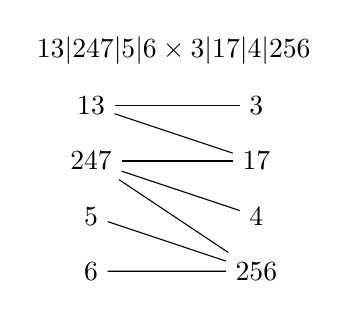
\begin{tikzpicture}[scale=.7]  
    \node (p) at (0, 0) {$13|247|5|6 \times 3|17|4|256$};
    \node (1) at (-1.5, -1) {$13$};
    \node (2) at (-1.5, -2) {$247$};
    \node (3) at (-1.5, -3) {$5$};
    \node (4) at (-1.5, -4) {$6$};
    %
    \node (5) at (1.5, -1) {$3$};
    \node (6) at (1.5, -2) {$17$};
    \node (7) at (1.5, -3) {$4$};
    \node (8) at (1.5, -4) {$256$};
    %
    \draw[-] (1)--(5); 
    \draw[-] (1)--(6); 
    \draw[-] (2)--(6); 
    \draw[-] (2)--(7); 
    \draw[-] (2)--(8); 
    \draw[-] (3)--(8); 
    \draw[-] (4)--(8);
    %
\end{tikzpicture}
\end{center}
Observe that the permutation can be read off the graph of the SCP by a vertical down slice through the edges of the graph.
\end{example}

As the intersection graph of any pair of essential complementary partitions is a bipartite tree, there is a unique path between any two vertices. 

\begin{notation}[Paths between blocks]
    For $(\sigma,\tau)$ a pair of essential complementary partitions, we denote by $\sigma_{i,j}$ (resp. $\tau_{i,j}$) the unique oriented path between blocks $\sigma_{i}$ and $\sigma_j$ (resp. $\tau_{i}$ and $\tau_j$).
\end{notation}
Note that we make a slight abuse in notation as the path $\sigma_{i,j}$ also depends on $\tau$.
We can immediately characterise the paths between adjacent blocks of $\SCP$s.

\begin{proposition} 
\label{lem:SCP-path-desc}
For any strong complementary pair $(\sigma,\tau)$, we have that
\begin{enumerate}
    \item $ \sigma_{i,i+1} = ( \min \sigma_i, \max \sigma_{i+1} )$ and $\min \sigma_i< \max \sigma_{i+1}$, 
    \item $  \tau_{i,i+1} =  ( \max \tau_i, \min \tau_{i+1} )$ and $\min \tau_{i+1}< \max \tau_{i}$.
\end{enumerate}
As a consequence, all strong complementary pairs are in both $\LAD$ and $\SUD$.
\end{proposition}
\begin{proof}
The path description of $(\sigma,\tau)$ is a straightforward observation. 
Since the minima of these paths are traversed from left to right, and the maxima from right to left, \cref{prop:LAD-ordered-EC} implies that strong complementary partitions are in both $\LAD$ and $\SUD$.
\end{proof}

%%%%%%%%%%%%%%%%%%%%%%%%%%%%%%%%%%%%%%%%%

\subsubsection{Subset shift and shift diagonals}

\begin{definition}[Subset shift operators]
\label{def:subset shifts}
Let $(\sigma,\tau) = (\sigma_1|\dots|\sigma_k,\tau_1|\dots|\tau_l)$ be an ordered partition pair, and let $M_i\subset (\sigma_{i} \ssm \min \sigma_{i})$ be a non-empty subset such that $\min M_i> \max \sigma_{i+1}$.
For this set we define the \emph{subset right shift operator} by
\begin{align*}
    R_{M_i}(\sigma) \eqdef \sigma_1|\dots|\sigma_i \ssm M_i|\sigma_{i+1} \cup M_i|\dots|\sigma_k
\end{align*}
Dually, let $M_{i+1}\subset (\tau_{i+1}\ssm \min \tau_{i+1})$  be a non-empty subset such that $\min M_{i+1}> \max \tau_{i}$.
For this set we define the \emph{subset left shift operator} by
\begin{align*}
    L_{M_{i+1}}(\tau) \eqdef \tau_1|\dots|\tau_i \cup M_{i+1}|\tau_{i+1} \ssm M_{i+1}|\dots|\tau_l \ .
\end{align*}
\end{definition}

\begin{example}
Performing the subset shifts $R_7$ and $L_{5,6}$ on the $\SCP$ $(\sigma,\tau)$ of \cref{ex:strong-complementary}, one obtains the pair $R_{7}(\sigma) \times L_{5,6}(\tau)$.
\begin{center}
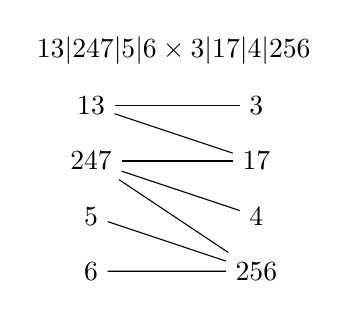
\begin{tikzpicture}[scale=.7]  
    \node (p) at (0, 0) {$13|247|5|6 \times 3|17|4|256$};
    \node (1) at (-1.5, -1) {$13$};
    \node (2) at (-1.5, -2) {$247$};
    \node (3) at (-1.5, -3) {$5$};
    \node (4) at (-1.5, -4) {$6$};
    %
    \node (5) at (1.5, -1) {$3$};
    \node (6) at (1.5, -2) {$17$};
    \node (7) at (1.5, -3) {$4$};
    \node (8) at (1.5, -4) {$256$};
    %
    \draw[-] (1)--(5); 
    \draw[-] (1)--(6); 
    \draw[-] (2)--(6); 
    \draw[-] (2)--(7); 
    \draw[-] (2)--(8); 
    \draw[-] (3)--(8); 
    \draw[-] (4)--(8);
    %
\end{tikzpicture}
\quad
\raisebox{3em}{$\xrightarrow{R_{7} \times L_{5,6}}$}
\quad
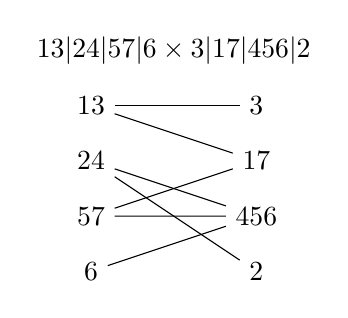
\begin{tikzpicture}[scale=.7]  
\node (p) at (0, 0) {$13|24|57|6 \times 3|17|456|2$};
\node (1) at (-1.5, -1) {$13$};
\node (2) at (-1.5, -2) {$24$};
\node (3) at (-1.5, -3) {$57$};
\node (4) at (-1.5, -4) {$6$};
%
\node (5) at (1.5, -1) {$3$};
\node (6) at (1.5, -2) {$17$};
\node (7) at (1.5, -3) {$456$};
\node (8) at (1.5, -4) {$2$};
%
\draw[-] (1)--(5); 
\draw[-] (1)--(6); 
\draw[-] (3)--(6); 
\draw[-] (2)--(7); 
\draw[-] (2)--(8); 
\draw[-] (3)--(7); 
\draw[-] (4)--(7);
%
\end{tikzpicture}
\end{center}
\end{example}

Observe that the left shift operator moves elements to the left, but acts on the right ordered partition.
Dually, the right shift operator moves elements to the right but acts on the left ordered partition.

\begin{remark}
    In the analogous description for the diagonal $\LAD$ obtained at the end of the Section \Guillaume{[REF]}, left and right shift operators act on the left and right ordered partitions, respectively. 
\end{remark}

For $p\geq 1$, let $\textbf{M} = (M_{i_1},\dots,M_{i_p}) \in [n]^{p}$, be such that $1\leq i_1 < i_2 \dots < i_p \leq k-1$, and each of the iterated compositions $R_\mathbf{M}(\sigma)  \eqdef  R_{M_{i_p}}\dots R_{M_{i_1}}(\sigma)$ are well-defined.
Similarly, for $q\geq 1$ let $\textbf{N} = (N_{i_q},\dots,N_{i_1}) \in [n]^{q}$ be such that $2\leq i_1 < i_2 \dots < i_q \leq k$, and each of the iterated compositions $L_\mathbf{N}(\tau)  \eqdef  L_{N_{i_1}}\dots L_{N_{i_q}}(\tau)$ are well-defined.
By convention, we allow the empty sequence of subset shift operators, which acts by the identity, i.e. define $R_{\mathbf{\emptyset}}(\sigma)  \eqdef  \sigma$ and $L_{\mathbf{\emptyset}} (\tau) \eqdef  \tau$.

\begin{definition}[Subset shift $\SU$ diagonal {\cite{SaneblidzeUmble04,saneblidzeComparingDiagonalsAssociahedra2022}}]
   The facets of the \emph{subset shift $\SU$ diagonal} are given by the formula
    \begin{align*}
        \SUD([n]) = \bigcup_{(\sigma,\tau)} \bigcup_{\mathbf{M}, \mathbf{N}} R_\mathbf{M}(\sigma)\times L_\mathbf{N}(\tau)
    \end{align*}
    where the unions are taken over all strong complementary partitions $(\sigma, \tau)$ of $[n]$, and on all well-defined sequences of shift operators $\textbf{M},\textbf{N}$.
\end{definition}

Let us now introduce an alternative definition, which will be proven in \cref{prop:subset shift to shift bijection} to be equivalent to the preceding one, and in \cref{prop: shift SUD and SUD are equal} to $\SUD$ with its $(I,J)$-description. 

\begin{definition}[Critical elements] \label{def:critical SU shift}
    Let $(\sigma,\tau)$ be a pair of ordered partitions.
    A \emph{critical element} is either an element $\rho \in (\sigma_i \ssm \min \sigma_i)$ such that $\rho>\max \sigma_{i,i+1}$, or an element $\rho \in (\tau_{i+1} \ssm \min\tau_{i+1})$ such that $\rho > \max \tau_{i,i+1}$. 
\end{definition}

Let us call \emph{critical} the right and left shift operators associated with the singleton sets given by critical elements, and denote them by $R_{\rho}$ and $L_{\rho}$.

\begin{definition}[Shift $\SU$ diagonal]
    The facets of the \emph{shift $\SU$ diagonal} are given by the formula
    \begin{align*}
        \SUD([n]) = \bigcup_{(\sigma,\tau)} \bigcup_{\mathbf{M}, \mathbf{N}} R_\mathbf{M}(\sigma)\times L_\mathbf{N}(\tau)
    \end{align*}
    where the unions are taken over all strong complementary partitions $(\sigma, \tau)$ of $[n]$, and on all well-defined sequences of critical shift operators $\textbf{M},\textbf{N}$.
\end{definition}

%\Guillaume{Do we keep the m-shifts?}

%However, we can actually relax the critical shift operator one step further \Kurt{make this the main def, then specialise to $m=1$ for prior proof}
%\begin{definition} \label{def:critical SU m shift}
%Let $(\sigma,\tau)$ be a pair of ordered partitions, and let $\rho \in (\sigma_i \ssm \min \sigma_i)$ such that $\rho>\max \sigma_{i,i+m}$, where $m\geq 1$, and similarly for $\tau$.
%For such elements we define the critical left and right $m$-shift operators to be
%\begin{eqnarray*}
 % R_\rho(\sigma) & = & \sigma_1|...|\sigma_i \ssm \rho|...|\sigma_{i+m} \sqcup \{\rho\}|...\sigma_k \\
 % L_\rho(\tau) & = & \tau_1|...|\tau_{i-m}\sqcup \rho|...|\tau_i \ssm \{\rho\}|...|\tau_l
%\end{eqnarray*}
%\end{definition}

%\begin{lemma}
%Any $m$-shift can performed by a sequence of $1$-shifts.
%\end{lemma}
%\begin{proof}
%Suppose for $m>0$ that we have, $\rho \in (\sigma_i \ssm \min \sigma_i)$ and $\rho> \max \sigma_{i,i+m}$.
%The we will show that there cannot be a $\sigma_{d,d+1}$ for $d\in [i,i+m-1]$ such that, all prior shifts of $\rho$ where well-defined, but this one fails.
%\begin{itemize}
 %   \item Simple property of SCPs and shifts conserving maximal elements of path
  %  \item Do a nice diagram to make it clear though \Kurt{todo see photo}
%\end{itemize}
%\end{proof}

%%%%%%%%%%%%%%%%%%%%%%%%%%%%%%%%%%

\subsubsection{First isomorphism: subset shift and shift}

We now make an interesting observation, whose proof is key to an equivalent definition of the subset shift $\SUD$ diagonal. 
\begin{proposition} 
\label{prop:SU-preserves-max}
The $\SU$ subset shift operators conserve the maximal element of paths.
In particular, for $(R_{\mathbf{M}}(\sigma),L_{\mathbf{N}}(\tau))$ a valid shift of an $\SCP$, we have that
\begin{align*}
    \max R_{\mathbf{M}}(\sigma)_{i,j} = \max \sigma_{i,j} \text{ and } \max L_{\mathbf{N}}(\tau)_{i,j} = \max \tau_{i,j}
\end{align*}
and consequently that
\begin{align*}
    \max R_{\mathbf{M}}(\sigma)_{i,i+1} = \max \sigma_{i+1} \text{ and } \max L_{\mathbf{N}}(\tau)_{i,i+1} = \max \tau_{i}  \ .
\end{align*}
\end{proposition}

\begin{proof}
We consider the right subset shift operator; the left subset shift operator proceeds similarly.
As $\SCP$s trivially meet the above conditions, we will prove the result inductively by assuming the result holds for $(R_{\mathbf{M}}(\sigma),L_{\mathbf{N}}(\tau))$, and then showing that applying a valid operator $R_{M_k}$ conserves the maximal elements of paths.
By the inductive hypothesis, we know that $\max R_{\mathbf{M}}(\sigma)_{k,k+1}= \max \sigma_{k+1}$.
As $R_{M_k}$ is a valid operator, we know two things.
Firstly $\min M_k > \max R_{\mathbf{M}}(\sigma)_{k+1}$.
Secondly, as $k$ is greater than the maximal index used by $\mathbf{M}$, we have that $\max \sigma_{k+1} = \max R_{\mathbf{M}}(\sigma)_{k+1}$.
So combining these we know that
\begin{align}\label{eq:shift-subset-dominates}
    \min M_k > \max R_{\mathbf{M}}(\sigma)_{k+1} = \max \sigma_{k+1} = \max R_{\mathbf{M}}(\sigma)_{k,k+1} \ . 
\end{align}
A key consequence of this inequality is that the corresponding graph of $(R_{M_k}R_{\mathbf{M}}(\sigma),L_{\mathbf{N}}(\tau))$ is a bipartite tree conditional on $(R_{\mathbf{M}}(\sigma),L_{\mathbf{N}}(\tau))$ being a bipartite tree: the shift will not disconnect the graph as none of the shifted elements are in the path $R_{\mathbf{M}}(\sigma)_{k,k+1}$. 
So, it is legitimate to speak of unique paths between blocks. 

We now explicitly explore how the shift operator $R_{M_k}$ alters paths. 
Throughout the rest of this proof, we use the following shorthand: we denote by $\delta_{k,k+1} \eqdef  R_{\mathbf{M}}(\sigma)_{k,k+1}$ the path between the adjacent blocks in $(R_{\mathbf{M}}(\sigma),L_{\mathbf{N}}(\tau))$, and by $\delta_{k+1,k}$ the same path reversed.
Let~$\gamma$ be any path between two blocks of $(R_{\mathbf{M}}(\sigma),L_{\mathbf{N}}(\tau))$, and let~$\gamma'$ be the path between the same blocks, by indices, in $(R_{M_k}R_{\mathbf{M}}(\sigma),L_{\mathbf{N}}(\tau))$. 
There are four cases to consider. 
\begin{enumerate}
    \item $\gamma$ does not contain an element of $M_k$.
    It is thus unaffected by the shift, so $\gamma' = \gamma$.

    \item $\gamma$ contains one element $m\in M_k$, i.e. it is of the form $\gamma = \alpha m \beta$, with $\alpha$ or $\beta$ possibly empty.
    Note that since $M_k$ defines a shift, $m$ is not in $\delta_{k,k+1}$, and $\delta_{k,k+1}$ is unaffected by the shift. 
    We assume that $m$ is incoming to $R_\mathbf{M}(\sigma)_{k}$, the case when it is outgoing is similar.
    We must have $\alpha \cap \delta_{k,k+1}=\emptyset$ since otherwise there would be an oriented loop from $R_\mathbf{M}(\sigma)_{k}$ to itself.
    For the same reason, $\beta \cap \delta_{k,k+1}$ must be connected and starting at $R_\mathbf{M}(\sigma)_{k}$.
    Then there are two cases to consider:
    \begin{enumerate}
        \item $\beta$ does not use any steps of $\delta_{k,k+1}$, in which case $\gamma' = \alpha m \delta_{k+1,k} \beta$.
        This is a path in the tree of $(R_{M_k}R_{\mathbf{M}}(\sigma),L_{\mathbf{N}}(\tau))$ with no repeated steps, as such it must be the unique minimal path. 
        
        \item $\beta$ uses steps of $\delta_{k,k+1}$, in which case $\gamma' = \alpha m (\delta_{k+1,k}\ssm \beta)(\beta \ssm \delta_{k+1,k})$.
        This follows, as we know that $\beta$ must follow the path $\delta_{k,k+1}$ for some time before diverging ($\beta$ could also be a subset of $\delta_{k,k+1}$, in which case it will never diverge).
        As such, the path $(\delta_{k+1,k}\ssm \beta)$ reaches the point of divergence from $R_{\mathbf{M}}(\sigma)_{k+1}$ instead of $R_{\mathbf{M}}(\sigma)_{k}$, then the path $(\beta \ssm \delta_{k+1,k})$ completes the rest of the route unchanged.

    \end{enumerate}
    \item $\gamma$ contains two elements of $M_k$. In which case we still have $\gamma'=\gamma$ (in path elements) but $\gamma'$ will step through the $(k+1)$th block instead of $\gamma$ stepping through the $k$th block, which imples that $\max \gamma=\max \gamma'$.
    
    \item $\gamma$ contains more than two elements of $M_k$. 
    This is impossible, as $\gamma$ would not be a minimal path on a tree.
\end{enumerate}
Observe all (non-trivial or non-contradictory) paths $\gamma'$ contain $m>\min M_k$ and either some addition or deletion by $\delta_{k,k+1}$.
It thus follows from \cref{eq:shift-subset-dominates} that $\max \gamma' = \max \gamma$: in each case, the maximal element will either be $m$, or in $\alpha$, or in $\beta$.
\end{proof}

The key result of the inductive proof was the chain of inequalities which yielded $\min M_k > \max R_{\mathbf{M}}(\sigma)_{k,k+1}$ (\cref{eq:shift-subset-dominates}).
It turns out, if we assume the inequality holds, we can drop the assumption that $k$ is greater than the maximal index used by $\mathbf{M}$, and the assumption that $\min M_k > \max R_{\mathbf{M}}(\sigma)_{k+1}$. 
Furthermore, once we have dropped the assumption that we need to perform shifts in an increasing order, we can generate all subset shifts by chains of singleton set shifts. This motivated the definition \cref{def:critical SU shift}.

As we have assumed the necessary feature of the proof of \cref{prop:SU-preserves-max}, we have the immediate corollary.

\begin{corollary} \label{cor: SU shift conserves maximal element of paths}
The critical left and right shift operators conserve the maximal element of paths, and if $(\sigma',\tau')$ is generated from critical shifts of $(\sigma,\tau) \in SCP$ then,
\begin{align*}
    \max \sigma'_{i,i+1} = \max \sigma_{i+1} \text{ and } \max \tau'_{i,i+1} = \max \tau_{i}
\end{align*}
\end{corollary}

\begin{definition}
The facets of the shift $\SUD$ are $\SCP$s, and their image under iterated applications of critical left and right shift operators.
\end{definition}

As one might suspect given the above corollaries.

\begin{proposition}\label{prop:subset shift to shift bijection}
The subset shift, and shift definitions of the $\SUD$ diagonal coincide.
\end{proposition}

\begin{proof}
We analyse the right shift operator, the case of the left shift is similar. 
First, we observe that any subset right shift $R_{M_k}(\sigma)$ can be decomposed in a series of right shifts: since $\min M_k > \max \sigma_{k,k+1}$ by the proof of \cref{prop:SU-preserves-max}, we can first shift $\min M_k$ to the right, then $\min (M_k \ssm \min M_k)$, and so on until the entire subset $M_k$ has been shifted to the right. 
This shows that any facet of the subset shift $\SUD$ diagonal is also a facet in the shift $\SUD$ diagonal
\\\\
For the reverse inclusion, we proceed by induction. We are required to show that if we apply a critical right shift to $(R_{\mathbf{M}}(\sigma),L_{\mathbf{N}}(\tau))$, say $(R_{\rho}R_{\mathbf{M}}(\sigma),L_{\mathbf{N}}(\tau))$, then this can be re-expressed as a well-defined subset shift operation i.e. $(R_{\mathbf{M'}}(\sigma),L_{\mathbf{N}}(\tau))$. Suppose that prior to the critical shift that $\rho$ lives in block $l$, then we must have
\begin{align*}
    1 \leq i_1 < \dots < i_j \leq l < i_{j+1} <\dots< i_d \leq k-1
\end{align*}
for some $j\in [d]$. If $i_j < l$, then $R_{\rho}R_{\mathbf{M}}(\sigma) = R_{M_{i_d}}\dots R_{\{\rho\}_{l}}R_{M_{i_j}}\dots R_{M_{i_1}}(\sigma)$, and we are done.
Otherwise, if $i_j = l$, let $M'_{i_j} = M_{i_j} \cup \{\rho \}$. It is clear that $R_{\rho}R_{\mathbf{M}}(\sigma) = R_{M_{i_d}}\dots R_{M'_{i_j}}\dots R_{M_{i_1}}(\sigma)$, however, we need to check that $R_{M'_{i_j}}$ is a well-defined subset operator. 
We know the subset shift operators will never move the minimal element, so $\rho > \min R_{\mathbf{M}}(\sigma)_{i_j}= \min (R_{M_{i_{j-1}}}\dots R_{M_{i_1}}(\sigma))_{i_j}$.
Then from \cref{cor: SU shift conserves maximal element of paths}, we know that $\rho>\max \sigma_{i_j+1} = \max (R_{M_{i_{j-1}}}\dots R_{M_{i_1}}(\sigma))_{i_j + 1}$, where the equality follows as $i_1<\dots<i_{j-1}<i_j$. This proves that $R_{M'_{i_j}}$ is well-defined, completing the inductive proof.
\end{proof}

%%%%%%%%%%%%%%%%%%%%%%%%%%%%%%%%%%%%%%

\subsubsection{Second isomorphism: shift and $(I,J)$ coincide}

The remainder of this section is devoted to the proof that the shift $\SUD$ diagonal is equal to the $\SUD$ diagonal. 

Given our existing theory, the closure of the critical shift operator is easy to establish.
\begin{lemma} \label{lem:SUD closed under shifts}
Let $(\sigma,\tau)\in \SUD$, if we apply a critical shift operator to it, then we remain in $\SUD$.
\end{lemma}
\begin{proof}
We consider just the right shift, and the left proceeds similarly. 
\cref{cor: SU shift conserves maximal element of paths} shows that the maxima of paths between consecutive vertices in $(R_{\rho}(\sigma),\tau)$ are the same as the ones in $(\sigma,\tau)$. 
Thus, all maxima of paths in $(R_{\rho}(\sigma),\tau)$ are traversed from right to left, and hence by \cref{prop:SUD are ordered EC}, we have that $(R_{\rho}(\sigma),\tau) \in \SUD$.   
\end{proof}

We now need to develop the theory of inverse shift operators.

\begin{definition}
Let $(\sigma,\tau)$ be a pair of ordered partitions $[n]$, we say that $(x,y)$, where $x<y$, is an \emph{inversion} if $x$ appears before $y$ in $\sigma$ and $y$ appears before $x$ in $\tau$. 
\end{definition}

\begin{proposition}
\label{p:crossings}
The set of inversions of a $\SUD$ facet is in bijection with its set of edge crossings. 
Moreover, the set $\SCP$ is equal to the set of facets with no crossings.
\end{proposition}

\begin{proof}
For the first part of the statement, it is clear that every inversion gives rise to a crossing. 
For the converse, one needs to check that an anti-inversion, where $y$ appears before $x$ in $\sigma$ and $x$ appears before $y$ in $\tau$, cannot occur in a facet of $\SUD$; this follows immediately from the $(I,J)$-conditions for $|I|=|J|=1$. 
The second part of the statement follows from the fact that facets of the diagonal with no crossings are in bijection with permutations.
As explained above, from a partition one obtains a strong complementary pair, which is in $\SUD$. 
In the other way around, given a strong complementary pair, one can read-off the partition in the associated tree, which has no crossings, by a vertical down-slice of edges, see \cref{ex:strong-complementary}.
\end{proof}
We say that an edge crossing is an \emph{adjacent crossing} if the two crossing elements are in adjacent blocks (i.e. $\sigma_i|\sigma_{i+1}$ or $\tau_i|\tau_{i+1}$).
\begin{lemma}
A facet $(\sigma,\tau) \in \SUD$ has a crossing if, and only if, it has an adjacent crossing.
\end{lemma}
\begin{proof}
An adjacent crossing is clearly a crossing. In the other direction, suppose there is a crossing between an element of $\sigma_i$ and an element of $\sigma_j$. If $\sigma_i$ and $\sigma_j$ are not adjacent, then the 'triangle' produced by the crossing elements encloses other $\sigma_k$ such that $i<k<j$, and this produces other crossings. We may repeat this process until end an adjacent crossing.
\end{proof}

We now define inverse critical shift operators.
\begin{definition} \label{def:critical SU inverse shift}
Let $(\sigma,\tau)$ be a pair of ordered partitions. Let $\rho \in \sigma_{i+1}$ be such that $\rho>\max \sigma_{i,i+1}$ and $(\alpha,\rho)$ is an adjacent crossing, where $\alpha$ is an arbitrary element which is smaller than $\rho$. 
Similarly, let $\rho \in \tau_{i} $ such that $\rho > \max \tau_{i,i+1}$ and $(\alpha,\rho)$ is an adjacent crossing.
Subject to these constraints, we informally define the inverse left/right shift operators as, $R^{-1}_\rho$ returns $\rho$ to $\sigma_i$, and $L^{-1}_\rho$ returns $\rho$ to $\tau_{i+1}$
\end{definition}
The theory of these inverse operators behaves as one would expect. We only develop the necessary results to prove the equality of the diagonals. 
\begin{lemma} \label{lem: shift operators are inverse to their inverses}
The shift operators are the inverses of the inverse shift operators.
\end{lemma}
\begin{proof}
If we apply a well-defined inverse shift operator $R^{-1}_{\rho}$ to $(\sigma,\tau)$, then we have $\alpha,\rho \in R^{-1}_{\rho}(\sigma)_{i}$ such that $\min R^{-1}_{\rho}(\sigma)_i \leq \alpha<\rho$ and $\rho >\max R^{-1}_{\rho}(\sigma)_{i,i+1}$. As such, $R_{\rho}$ is well-defined, and $R_{\rho} R^{-1}_{\rho}=id$. A similar result holds for the left operator.
\end{proof}

\begin{lemma}
The inverse shift operators conserve the maximal elements of paths.
\end{lemma}
\begin{proof}
This is an immediate corollary of the prior lemma, and the fact that the shift operators conserves maximal elements of paths (\cref{prop:SU-preserves-max}).
\end{proof}

\begin{lemma} \label{lem:SUD closed under inverse shifts}
Let $(\sigma,\tau)\in \SUD$, if we apply an inverse critical shift operator to it, then we remain in $\SUD$.
\end{lemma}
\begin{proof}
As in \cref{lem:SUD closed under shifts}, as the inverse shift operators conserve the maxima of paths, and these same maxima continue to be traversed from right to left, it follows by \cref{prop:SUD are ordered EC} that the output of an inverse shift operator will remain in $\SUD$.
\end{proof}

\begin{lemma}\label{lem:inductive decomposition into SCP}
All $(\sigma,\tau)\in \SUD$ are mapped to a $\SCP$ by a finite number of inverse shifts.
\end{lemma}
\begin{proof}
It is immediate that given any element, $(\sigma,\tau) \in \SUD$ then we will only be able to apply a finite chain of inverse shift operators to it before no further operations are available. (It is straightforward to show each inverse shift decreases the number of crossings. An even simpler argument is, there are only a finite number of elements to move by a finite number of blocks).
\\\\
We now illustrate how to identify an inverse shift for the cases of the following partition.
\begin{enumerate}
    \item All adjacent blocks are connected by paths of length $2$
    \item There exist adjacent blocks which are connected by a path of length $2k$ for $k>1$.
    \begin{enumerate}
        \item The maximal step of this path is not the last step.
        \item The maximal step of this path is the last step.
        \begin{enumerate}
            \item The $\tau$ block containing the maximal step is not the greatest block.
            \item The $\tau$ block containing the maximal step is the greatest block.
        \end{enumerate}
    \end{enumerate}
\end{enumerate}
In case $1$, if $\sigma,\tau$ is not an $\SCP$ then it must have a crossing, and hence an adjacent crossing. This adjacent crossing must be in one of the following two forms, and admits the following inverse shifts.
\begin{center}
\begin{tikzcd}
\sigma_i \arrow[rd,dash,"a"] & \cdot\\
\sigma_{i+1} \arrow[r,dash,"b"] \arrow[ru,dash,"{\rho}"] & \cdot
\end{tikzcd}
$\xrightarrow{R_\rho^{-1}}$
\begin{tikzcd}
\sigma_i \sqcup \rho \arrow[rd,dash,"a"] \arrow[r,dash,"{\rho}"]& \cdot\\
\sigma_{i+1}\ssm \rho \arrow[r,dash,"b"]  & \cdot
\end{tikzcd}
\quad
\begin{tikzcd}
\cdot \arrow[rd,dash,"a"] \arrow[r,dash,"b"]& \tau_{i-1}\\
\cdot  \arrow[ru,dash,"{\rho}"] & \tau_{i}
\end{tikzcd}
$\xrightarrow{L_\rho^{-1}}$
\begin{tikzcd}
\cdot \arrow[rd,dash,"a"] \arrow[r,dash,"b"]& \tau_{i-1} \ssm \rho\\
\cdot  \arrow[r,dash,"{\rho}"] & \tau_{i} \sqcup \rho
\end{tikzcd}

\end{center}
\Kurt{Better diagrams}
Both shifts are well-defined, as in each case the first order $I,J$ conditions witness that $a<b<\rho$.
\\\\
In case $2.a$, consider the adjacent blocks say $\sigma_i|\sigma_{i+1}$ (the $\tau$ case is similar), let $\rho=\max \sigma_{i,i+1}$, and let $m\geq 1$ be such that $\rho$ steps into $\sigma_{i+1+m}$. We know that $m\geq 1$ due to the $\SUD$ order, i.e. $\max \sigma_{i,i+1+m} = \rho$ implies that $\sigma_{i,i+1+m}$ comes after $\sigma_{i}$, and by assumption after $\sigma_{i+1}$. Then using squiggly lines to denote paths of length $\geq 1$ we have,
\begin{center}
\begin{tikzcd}
\sigma_i \arrow[r,squiggly,dash] & \cdot\\
\sigma_{i+1} \arrow[r,squiggly,dash] & \cdot\\
\sigma_{i+1+m} \arrow[ruu,dash, "\rho"] \arrow[ru,squiggly,dash]
\end{tikzcd}
$\xrightarrow{R_\rho^{-1}}$
\begin{tikzcd}
\sigma_i \arrow[r,squiggly,dash] & \cdot\\
\sigma_{i+1} \sqcup \rho \arrow[r,squiggly,dash] \arrow[ru,dash, "\rho"]& \cdot\\
\sigma_{i+1+m} \ssm \rho \arrow[ru,squiggly,dash]
\end{tikzcd}
\end{center}
As $\rho=\max \sigma_{i,i+1} > \max\sigma_{i+1+m,i+1}$ the shift operation is well defined.
\\\\
In the case $2.b.i.$, there exists $j,m>0$ such that $\tau_{j-m}$ is the $\tau$ block which contains the maximal element $\rho$, and $\tau_j$ is any greater block on the path from $\sigma_i$ to $\sigma_{i+1}$. Then we may apply the following inverse shift operator.
\begin{center}
\begin{tikzcd}
\sigma' \arrow[r,squiggly,dash] \arrow[rd,squiggly,dash]& \tau_{j-m}\\
\sigma_{i} \arrow[r,squiggly,dash] & \tau_j\\
\sigma_{i+1} \arrow[ruu,dash, "\rho"] 
\end{tikzcd}
$\xrightarrow{L_\rho^{-1}}$
\begin{tikzcd}
\sigma' \arrow[r,squiggly,dash] \arrow[rd,squiggly,dash]& \tau_{j-m}\setminus \rho\\
\sigma_{i} \arrow[r,squiggly,dash] & \tau_j \sqcup \rho\\
\sigma_{i+1} \arrow[ru,dash, "\rho"] 
\end{tikzcd}
\end{center}
Consider case $2.b.ii$ (this does exist, e.g. $12|3|4 \times 23|14$). 
Then,
\begin{itemize}
    \item We know each $\sigma'$ must be above $\sigma_{i+1}$ due to the maximal element $\rho$ being the last step.
    \item This also tells us each $\sigma'$ is above $\sigma_i$.
    \item So if the path $\sigma_{i,i+1} = (i_1,j_1,i_2,...,i_{k},j_k)$ where $j_k = \rho$ then
    \item $\max \{i_1,...,i_k\} <\max \{j_1,...,j_k\} =: \rho$, and $\rho':=\max \{i_1,...,i_{k-1}\} > \max \{j_1,...,j_{k-1}\} $. That is to say that $\rho'$ witnesses the second last $\sigma$ block being before $\sigma_i$.
    \item Suppose that $\rho' < i_{k}$. This implies that $j_{k-1}< i_k$. Then, by the first order $I,J$ condition, the $\sigma$ block which contains $i_k,j_{k-1}$ forces the $\tau$ block containing $j_{k-1}$ to be greater than the $\tau$ block containing $i_k$ (and also containing $\rho$). This is a contradiction.
    \item So we know that $\rho'>i_{k}$.
    \item The path $(i_{k},j_{k-1},...,\rho')\setminus \rho'$ connects the $\tau$ block which contains $\rho$  to the $\tau$ block which contains $\rho'$. 
    Let $j$ and $m$ be indices such that $\rho \in \tau_j$ and $\rho' \in \tau_{j-m}$. 
    \item By assumption, $m >0$ as $\tau_j$ is the greatest $\tau$ block.
    \item Hence, by construction $\max \tau_{j,j-m} < \rho'$, so $L_{\rho'}^{-1}$ is a valid inverse shift, which returns $\rho'$ to $\tau_j$.
\end{itemize}
\end{proof}

\begin{example}
\Kurt{I can do an example for each of the cases if this is the route we take}
\begin{enumerate}
    \item 
    \item 
    \begin{enumerate}
        \item 
        \item 
        \begin{enumerate}
            \item 
            \item $12|3|4\times 23|14 \xrightarrow{L_{3}^{-1}} 12|3|4\times 2|134$ 
        \end{enumerate}
    \end{enumerate}
\end{enumerate}
\end{example}

\begin{proposition} \label{prop: shift SUD and SUD are equal}
    The facets of shift $\SUD$ and $\SUD$ are equal.
\end{proposition}
\begin{proof}
    We first note that $\SCP$s are known elements of $\SUD$ and shift $\SUD$.
    The proof that every facet of shift $\SUD$ is in $\SUD$ follows from the closure of $\SUD$ under the shift operator (\cref{lem:SUD closed under shifts}).
    The proof that every facet of $\SUD$ is in shift $\SUD$ follows from the closure of $\SUD$ under the inverse shift operator (\cref{lem:SUD closed under inverse shifts}) and an inductive argument that decomposes any facet into a $\SCP$ through inverse shift operators (\cref{lem:inductive decomposition into SCP}).
    As shift operators are the inverse of the inverse shift operators (\cref{lem: shift operators are inverse to their inverses}), for any given $\SUD$ facet, this provides a $\SCP$ and a sequence of shifts to form it, showing it is a shift $\SUD$ facet.
\end{proof}

%%%%%%%%%%%%%%%%%%%%%%%%%%%%%%%%%%%%%%%%%%

\subsubsection{Some consequences}

Combinining \cref{prop:subset shift to shift bijection} and \cref{prop: shift SUD and SUD are equal}, we obtain that

\begin{theorem}
    Subset shift $\SU$ and $\SUD$ coincide.
\end{theorem}

This
\begin{enumerate}
    \item resolves a conjecture of \cite{LA21} for the operahedra, and a conjecture of \cite{MazuirLA22} for the multiplihedra;
    \item provides a new proof that all known diagonals on the associahedra coincide \cite{saneblidzeComparingDiagonalsAssociahedra2022}
\end{enumerate}
Moreover, this allows us to obtain alternative descriptions of all four operadic diagonals, in particular
\begin{enumerate}
    \item subset shift and shift definitions of $\LA$ diagonal,
    \item matrix description of $\LA$ diagonal,
    \item conjectural description as subdivision of the cube [...]
\end{enumerate}
The next subsection is devoted to such a translation. 
One could hope for similar results in the case of the freehedra [REFS].

%%%%%%%%%%%%%%%%%%%%%%%%%%%%%%%%%%%%%%%%%%

\subsubsection{Shifts Under the Face Poset Isomorphism}

\begin{lemma}
The critical left and right shift operators send a facet of $\SUD$ to an adjacent facet of $\SUD$. This can be interpreted as stepping through a shared facet of the facets.
\end{lemma}
\begin{proof}
Let $(\sigma_1|\dots|\sigma_k,\tau) \in \SUD$, and let $\rho \in \sigma_{i}$ be a critical element. Then, the shift operator $R_{\rho}$ steps from the facet $(\sigma_1|\dots|\sigma_i |\sigma_{i+1} |\dots|\sigma_k, \tau)$, to the facet $(\sigma_1|\dots|\sigma_i \ssm \{\rho\}|\sigma_{i+1} \sqcup \{\rho\}|\dots|\sigma_k,\tau)$, through the facets of facets $(\sigma_1|\dots|\sigma_i \ssm \{\rho\}|\rho|\sigma_{i+1}|\dots|\sigma_k, \tau)$.
\end{proof}

As such, an immediate corollary of $\theta:\LAD \to \SUD$ being a face poset isomorphism is that their are analogous critical shift definitions of $\LAD$ induced by $\theta^{-1}$. 
We now explicitly state the critical shift $\LAD$ definition.
\begin{definition} \label{def:critical LA shift}
Let $(\sigma,\tau)$ be a pair of ordered partitions, and let $\rho \in (\sigma_{i+1} \ssm \max \sigma_{i+1})$ such that $\rho< \min \sigma_{i,i+1}$. Such an element $\rho$ is said to be \emph{critical}. 
We similarly define the critical elements of $\tau$ to be, $\rho \in (\tau_{i} \ssm \max\tau_{i})$ such that $\rho < \min \tau_{i,i+1}$. 
We define the left shift operator $L_{\rho}$ to act on $\sigma$, and the right shift $R_{\rho}$ operator to act on $\tau$.
\end{definition}
We note that compared to shift $\SUD$, the left shift operator now acts on the left ordered partition, and the right shift operator on the right ordered partition, a distinct notational improvement.
The correctness of this definition can be verified directly by obvious variants of the proofs of this section for the $\LAD$ diagonal.
There is also a clear translation of the subset shift operator, which we will not write out in full. 
We now explore in example how the $\LAD$ shift structure is induced by $\theta$.

\begin{example} \label{ex:shift translation by theta}
The $\SCP$s $(\sigma,\tau)  \eqdef  5|17|4|236 \times 57|146|3|2$, and $(\sigma',\tau')  \eqdef  13|247|5|6 \times 3|17|4|156$, are in bijection through $\theta$. Graphically this bijection has a clear symmetry,
\begin{center}
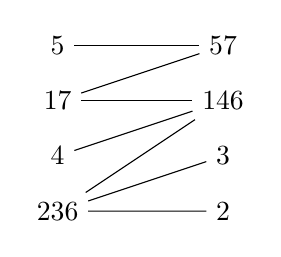
\begin{tikzpicture}[scale=.7]  
\node (1) at (-1.5, -1) {$5$};
\node (2) at (-1.5, -2) {$17$};
\node (3) at (-1.5, -3) {$4$};
\node (4) at (-1.5, -4) {$236$};
%
\node (5) at (1.5, -1) {$57$};
\node (6) at (1.5, -2) {$146$};
\node (7) at (1.5, -3) {$3$};
\node (8) at (1.5, -4) {$2$};
%
\draw[-] (1)--(5); 
\draw[-] (2)--(5); 
\draw[-] (2)--(6); 
\draw[-] (3)--(6); 
\draw[-] (4)--(6); 
\draw[-] (4)--(7); 
\draw[-] (4)--(8);
%
\end{tikzpicture}
$\xrightarrow{\theta}$
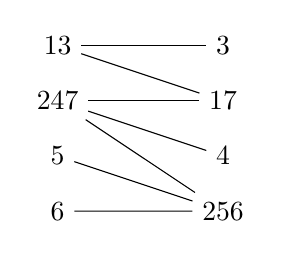
\begin{tikzpicture}[scale=.7]  
\node (1) at (-1.5, -1) {$13$};
\node (2) at (-1.5, -2) {$247$};
\node (3) at (-1.5, -3) {$5$};
\node (4) at (-1.5, -4) {$6$};
%
\node (5) at (1.5, -1) {$3$};
\node (6) at (1.5, -2) {$17$};
\node (7) at (1.5, -3) {$4$};
\node (8) at (1.5, -4) {$256$};
%
\draw[-] (1)--(5); 
\draw[-] (1)--(6); 
\draw[-] (2)--(6); 
\draw[-] (2)--(7);
\draw[-] (2)--(8); 
\draw[-] (3)--(8); 
\draw[-] (4)--(8);
%
\end{tikzpicture}
\end{center}
We now illustrate all possible $\LAD$ shifts of the left $\SCP$ and all possible $\SUD$ shifts of the right $\SCP$. We first display how the $\LAD$ left shifts act on $\sigma$, and the $\SUD$ left shifts act on $\tau'$. We indicate shifts by their corresponding critical element, drawing them to avoid crossings, and so they align with their isomorphic shift under $\theta$.
\begin{center}
{\small
\begin{tikzcd}
& 5|17|4|236 \arrow[ld,"p=3"] \arrow[d,"p=1"] \arrow[rd,"p=2"]\\
5|17|34|26 \arrow[rd,"p=1"] \arrow[d,"p=2"]&
15|7|4|236  \arrow[rd,"p=2"] \arrow[d,"p=3"]&
5|17|24|36 \arrow[d,"p=1"]\\
5|17|234|6 \arrow[d,"p=1"]&
15|7|34|26  \arrow[dl,"p=2"]&
15|7|24|36  \\
15|7|234|6 
\end{tikzcd}
\begin{tikzcd}
& 3|17|4|256 \arrow[ld,red,"p=5"] \arrow[d,"p=7"] \arrow[rd,"p=6"]\\
3|17|45|26 \arrow[rd,"p=7"] \arrow[d,red,"p=6"]&
37|1|4|256 \arrow[rd,"p=6"] \arrow[d,"p=5"]&
 3|17|46|25 \arrow[d,"p=7"]\\
3|17|456|2 \arrow[d,"p=7"]&
37|1|56|24 \arrow[dl,"p=6"]&
37|1|46|25 \\
37|1|456|2
\end{tikzcd}
}
\end{center}
The possible $\LAD$ right shifts (acting on $\tau$)  are,
\begin{center}
\begin{tikzcd}
\sigma \times 57|146|3|2 \arrow[r,"p=1"] & \sigma \times 57|46|13|2 \arrow[r,"p=1"] & \sigma \times 57|46|3|12
\end{tikzcd}
\end{center}
The possible $\SUD$ right shifts (acting on $\sigma'$) are,
\begin{center}
\begin{tikzcd}
13|247|5|6 \times \tau' \arrow[r,"p=7"] & 13|24|57|6 \arrow[r,"p=7"] \times \tau' & 13|24|5|67 \times \tau'
\end{tikzcd}
\end{center}
We note that as the left and right shifts (for both diagonals) can be performed independently, we could combine these lattices into a product of lattices. 
No other shifts are possible, observe for instance that we cannot perform the $\LAD$ left shift $15|7|234|6 \times 57|46|13|2 \xrightarrow{p=2} 15|27|34|6 \times 57|46|13|2$ as the minimal path connecting $234$ and $7$ contains $1$ which is smaller than $2$ (see \cref{ex:ECbijection}).
As an example of a $\SUD$ subset shift, and the bijection to critical shifts (\cref{prop:subset shift to shift bijection}), we observe that the unique way of producing $13|247|5|6 \times 37|1|456|2$ from subset shifts is given by
\begin{center}
\begin{tikzcd}
13|247|5|6 \times 3|17|4|256 \arrow[r,"{R_{\{5,6\}}}"] & 13|247|5|6 \times 3|17|456|2 \arrow[r,"{R_{\{7\}}}"] & 13|247|5|6 \times 37|1|456|2
\end{tikzcd}
\end{center}
This corresponds to combining the critical right shift operators of the $\SUD$ diagonal which have been indicated in red into a single subset.
We note it is also possible to apply $\SUD$ shifts to $(\sigma,\tau)$ and $\LAD$ shifts to $(\sigma',\tau')$. 
\end{example}

\Kurt{Mention the LAD and SUD shifts generate the (same) facets of the hexagon in two different ways.}

We have the following equivalent characterisations of the $\LAD$ and $\SUD$ diagonals. \Kurt{Probably in the intro somewhere}
\begin{itemize}
    \item $I,J$ conditions
    \item As orderings of essential complementary partitions
    \item Subset shift
    \item Critical element shift
    \item Matrix
    \item Cubical?
\end{itemize}








%%%%%%%%%%%%%%%%%%%%%%%%%%%%%%%%%%%

\section{Topological operadic structures}

\subsection{Operadic diagonals on the operahedra and multiplihedra}

The permutahedra are part of a more general family of polytopes called Loday realizations of the \emph{operahedra} \cite[Def. 2.9]{LA21} which encodes the notion of homotopy operad \cite[Def. 4.11]{LA21}.
For every planar tree $t$, there is a corresponding polytope $P_t$ whose codimension $k$ faces are in bijection with nestings of $t$ with $k$ non-trivial nests.
Since the operahedra are generalized permutahedra \cite[Cor. 2.16]{LA21}, a choice of diagonal for the permuthedra induces a choice of diagonal for every operahedron \cite[Cor. 1.31]{LA21}.
Every face of an operahedron is isomorphic to a product of lower-dimensional operahedra, via an isomorphism $\Theta$ which generalizes the one above, see Point (5) of \cite[Prop. 2.3]{LA21}.

\begin{definition}
    An \emph{operadic diagonal} for the operahedra is a choice of diagonal $\triangle_t$ for each operahedron~$P_t$, such that $\triangle:=\{\triangle_t\}$ commutes with the map $\Theta$, i.e. it satisfies \cite[Prop. 4.14]{LA21}.
\end{definition}

\begin{theorem}[Operadic structures on the operahedra] 
    \label{thm:operahedra}
There are exactly 
\begin{enumerate}
    \item four operadic diagonals of the Loday operahedra, therefore exactly
    \item four colored topological cellular operad structures on the Loday operahedra, and incidentally exactly
    \item four universal tensor products of homotopy operads,
\end{enumerate}
two of which (the $\LA$ and $\SU$ diagonals) agree with the generalized Tamari order on fully nested trees. 
\end{theorem}

\begin{proof}
    Let us first examine Point (1).
    By \cref{prop:unique-operad}, we know that if one of the four choices $\LAD, (\LAD)^\op, \SUD, (\SUD)^\op$ is made on an operahedron $P_t$, one has to make the same choice on every lower-dimensional operahedron appearing in the decomposition $P_{t_1} \times \cdots \times P_{t_k} \cong F \subset P_t$ of a face $F$ of $P_t$. 
    Now suppose that one makes two distinct choices for two operahedra $P_t$ and $P_{t'}$.
    It is easy to find a bigger tree $t''$ of which both $t$ and $t'$ are subtrees.
    Therefore, $P_t$ and $P_{t'}$ appear as facets of $P_{t''}$ and by the preceding remark, any choice of diagonal for $P_{t''}$ will then contradict our initial two choices. 
    Thus, these had to be the same from the start, which concludes the proof. 

    Point (2) then follows from fact that a choice of diagonal for the Loday realizations of the operahedra \emph{forces} a unique topological cellular colored operad structure on them, see \cite[Theorem 4.18]{LA21}.
    Since universal tensor products of homotopy operads are induced by a colored operad structure on the operahedra \cite[Cor. 4.24]{LA21}, we obtain Point~(3).
    Finally, since only vectors with strictly descreasing coordinates induce the generalized Tamari order on the $1$-skeleton of the operahedra \cite[Prop. 3.11]{LA21}, we get the last part of the statement. 
\end{proof}

This answers the first question in \cite[Remark 3.14]{LA21}.

Two other important families of generalized permutahedra are the \emph{Loday associahedra} and \emph{Forcey--Loday multiplihedra}, which encode respectively $\Ainf$-algebras and $\Ainf$-morphisms \cite[Prop. 4.9]{MazuirLA22}, as well as $\Ainf$-categories and $\Ainf$-functors \cite[Section 4.3]{MazuirLA22}.
Using the same techniques as in the case of the operahedra, they were endowed with diagonals and compatible operad and operadic bimodule structures in \cite[Theorem~1]{MazuirLA22}.
An analogous notion of \emph{operadic diagonal} is available for these polytopes, see \cite[Proposition 2.14]{MazuirLA22}.

\begin{samepage}
\begin{theorem}[Operadic structures on the multiplihedra]
There are exactly 
\begin{itemize}
    \item four operadic diagonals of the Forcey--Loday multiplihedra, therefore exactly
    \item four topological cellular operadic bimodule structures (over the Loday associahedra) on the Forcey--Loday multiplihedra, and incidentally exactly
    \item four compatible universal tensor products of $\Ainf$-algebras and $\Ainf$-morphisms,
\end{itemize}
two of which (the $\LA$ and $\SU$ diagonals) agree with the Tamari(-type) order on ($2$-colored) planar trees. 
\end{theorem}
\end{samepage}

\begin{proof}
    The proof is similar to the one of \cref{thm:operahedra}, using the results of \cite{MazuirLA22}.
\end{proof}

We shall see now that these different operadic structures are related to one another in the strongest possible sense: they are all isomorphic as topological cellular operadic structures.

%%%%%%%%%%%%%%%%%%%%%%%%%%%%%%%%%%%


\subsection{Relating operadic diagonals} 


%In this section we show that the four diagonals are isomorphic, and that this induces an isomorphism of the corresponding operadic structures on the operahedra, multiplihedra and associahedra.

Recall that the topological cellular operad structure on the operahedra \cite[Def. 4.17]{LA21} is given by a family of partial composition maps 
\[
\vcenter{\hbox{
\begin{tikzcd}[column sep=1cm]
\circ_i^{\LA}\ : \ P_{t'}\times P_{t''}
\arrow[r,  "\tr\times \id"]
& P_{(t',\omega)}\times P_{t''}
 \arrow[r,hookrightarrow, "\Theta"]
&
P_t \ .
\end{tikzcd}
}}  \]
Here, the map $\tr$ is the \emph{unique} topological cellular map which commutes with the diagonal~$\LAD$ \cite[Prop. 7]{masudaDiagonalAssociahedra2021}. 
This partial composition $\circ_i^\LA$ is an isomorphism (in the category $\PolySub$ \cite[Def. 4.13]{LA21}) between the product $P_{t'}\times P_{t''}$ and the facet $t' \circ_i^\LA t''$ of~$P_t$.
Using the $\SU$ diagonal $\SUD$, one can define similarly a topological operad structure via the same formula, but with a different transition map $\tr$, which commutes with $\SUD$.

Recall that a face $F$ of $P_t$ is represented by a nested tree $(t,\mathcal{N})$, which can be written uniquely as a sequence of substitution of trivially nested trees 
$(t,\mathcal{N})=t_1\circ_{i_1} t_2 \circ_{i_2} t_3 \cdots \circ_{i_k} t_{k+1}$.
Note that we do not need to specify a parenthesization of this sequence of $\circ_i$ operations since these form an operad \cite[Def. 4.7]{LA21}.
At the geometric level, we have an isomorphism
\[\circ_{i_1}^\LA \circ_{i_2}^\LA \cdots \circ_{i_k}^\LA: P_{t_1} \times P_{t_2} \times \cdots \times P_{t_{k+1}} \overset{\cong}{\longrightarrow} F \subset P_t \]
between a uniquely determined product of lower dimensional operahedra, and the face $F=(t,\mathcal{N})$ of~$P_t$.
Note that we can omit the parentheses in the sequence of $\circ_i^\LA$ operations since they define an operad structure \cite[Thm 4.18]{LA21}.
The same holds when taking the~$\circ_i^\SU$ operations instead of the $\circ_i^\LA$. 

\begin{definition}
    For any operahedron $P_t$, the map $\Psi_t : P_t \to P_t$ is defined 
    \begin{itemize}
        \item on the interior of the top face by the identity $\id : \mathring P_t \to \mathring P_t$, and 
        \item on the interior of the face $F=t_1 \circ_{i_1} t_2 \circ_{i_2} \cdots \circ_{i_k} t_{k+1}$ of~$P_t$ by the composition of the isomorphisms
        \[ 
        (\circ_{i_1}^\SU \circ_{i_2}^\SU \cdots \circ_{i_k}^\SU) (\circ_{i_1}^\LA \circ_{i_2}^\LA \cdots \circ_{i_k}^\LA)^{-1}: F \to F \ . \] 
    \end{itemize}
\end{definition}

\begin{proposition}
    \label{thm:top-iso}
    The map $\Psi:=\{\Psi_t\}$ is an isomorphism of topological cellular symmetric colored operad in the category $\PolySub$.
\end{proposition}

\begin{proof}
    By definition, we have that $\Psi$ is an isomorphism in the category $\PolySub$. 
    It remains to show that it preserves the operad structures, i.e. that the following diagram commutes
    \[
    \vcenter{\hbox{
    \begin{tikzcd}[column sep=2.2cm, row sep=1.3cm]
    P_{t'}\times P_{t''}
    \arrow[r,  "\circ_i^\LA"] 
    \arrow[d,  "\Psi_{t'}\times\Psi_{t''}"]
    & P_{t} \arrow[d,  "\Psi_t"] \\
    P_{t'}\times P_{t''}  
    \arrow[r,  "\circ_i^\SU"]
    & P_{t}\ .
    \end{tikzcd}
    }}\]
    For two interior points $(x,y) \in \mathring P_{t'}\times \mathring P_{t''}$, the diagram clearly commutes by definition, since $\Psi_{t'}$ $\Psi_{t''}$ are the identity in that case. 
    If $x$ is in a face $F=t_1 \circ_{i_1} t_2 \circ_{i_2} \cdots \circ_{i_k} t_{k+1}$ of the boundary of $P_{t'}$, then the lower composite is equal to $\circ_i^\SU (\circ_{i_1}^\SU \circ_{i_2}^\SU \cdots \circ_{i_k}^\SU \times \id)(\circ_{i_1}^\LA \circ_{i_2}^\LA \cdots \circ_{i_k}^\LA \times \id)^{-1}$, and so is the upper composite since $\Psi_t$ starts with the inverse $(\circ_i^\LA)^{-1}$ and the decomposition of $F$ unto $P_{t_1} \times \cdots \times P_{t_{k+1}} \times P_{t''}$ is unique.
    The case when $y$ is in the boundary of $P_{t''}$ is similar.  
    Finally, the compatibility of $\Psi$ with units and the symmetric group actions are straightfoward to check, see \cite[Def. 4.17 and Thm 4.18]{LA21}.
\end{proof}

Note that $\Psi$ is \emph{not} a morphism of ``Hopf" operads, i.e. it does not commute with the respective diagonals $\LAD$ and $\SUD$. 
\Guillaume{Give explicit counterexample}

\begin{corollary}
    The four topological operad structures on the operahedra are all isomorphic. 
\end{corollary}

\begin{proof}
    It is clear that the proof of \cref{thm:top-iso} does not depend on the specific choices of diagonals $\LAD$ and $\SUD$, it can therefore be applied to any pair of diagonals among $\LA, \LA^\op, \SU$ and $\SU^\op$. 
\end{proof}

\Guillaume{Find an iso which commutes??}

\begin{example}
    This isomorphism is a highly non-trivial map. 
    For instance, it is not the one you would expect...  [compare with the general symmetries]
\end{example}


\Guillaume{faire direct l'iso topologique, puis traduire?}


%%%%%%%%%%%%%%%%%%%%%%%%%%%%%%%%%%%

\section{Appendix: Shuffle trees}
